%%%%%%%%%%%%%%%%%%%%%%%%%%%%%%%%%%%%%%%%%
% Thesis 
% LaTeX Template
% Version 1.3 (21/12/12)
%
% This template has been downloaded from:
% http://www.latextemplates.com
%
% Original authors:
% Steven Gunn 
% http://users.ecs.soton.ac.uk/srg/softwaretools/document/templates/
% and
% Sunil Patel
% http://www.sunilpatel.co.uk/thesis-template/
%
% License:
% CC BY-NC-SA 3.0 (http://creativecommons.org/licenses/by-nc-sa/3.0/)
%
% Note:
% Make sure to edit document variables in the Thesis.cls file
%
%%%%%%%%%%%%%%%%%%%%%%%%%%%%%%%%%%%%%%%%%

%----------------------------------------------------------------------------------------
%	PACKAGES AND OTHER DOCUMENT CONFIGURATIONS
%----------------------------------------------------------------------------------------

\documentclass[10pt, a4paper, oneside]{Thesis} % Paper size, default font size and one-sided paper

\graphicspath{{./Pictures/}} % Specifies the directory where pictures are stored

\usepackage[square, authoryear, comma]{natbib} % Use the natbib reference package - read up on this to edit the reference style; if you want text (e.g. Smith et al., 2012) for the in-text references (instead of numbers), remove 'numbers' 
\usepackage{amsmath}
\hypersetup{urlcolor=blue, colorlinks=true} % Colors hyperlinks in blue - change to black if annoying
\title{\ttitle} % Defines the thesis title - don't touch this

\begin{document}

\frontmatter % Use roman page numbering style (i, ii, iii, iv...) for the pre-content pages

\setstretch{1.3} % Line spacing of 1.3

% Define the page headers using the FancyHdr package and set up for one-sided printing
\fancyhead{} % Clears all page headers and footers
\rhead{\thepage} % Sets the right side header to show the page number
\lhead{} % Clears the left side page header

\pagestyle{fancy} % Finally, use the "fancy" page style to implement the FancyHdr headers

\newcommand{\HRule}{\rule{\linewidth}{0.5mm}} % New command to make the lines in the title page

% PDF meta-data
\hypersetup{pdftitle={\ttitle}}	
\hypersetup{pdfsubject=\subjectname}
\hypersetup{pdfauthor=\authornames}
\hypersetup{pdfkeywords=\keywordnames}

%----------------------------------------------------------------------------------------
%	Superscript and subscript code
%----------------------------------------------------------------------------------------
 
\makeatletter
\newcommand\textsubscript[1]{\@textsubscript{\selectfont#1}}
\def\@textsubscript#1{{\m@th\ensuremath{_{\mbox{\fontsize\sf@size\z@#1}}}}}
\newcommand\textbothscript[2]{%
  \@textbothscript{\selectfont#1}{\selectfont#2}}
\def\@textbothscript#1#2{%
  {\m@th\ensuremath{%
    ^{\mbox{\fontsize\sf@size\z@#1}}%
    _{\mbox{\fontsize\sf@size\z@#2}}}}}
\def\@super{^}\def\@sub{_}
\catcode`^\active\catcode`_\active
\def\@super@sub#1_#2{\textbothscript{#1}{#2}}
\def\@sub@super#1^#2{\textbothscript{#2}{#1}}
\def\@@super#1{\@ifnextchar_{\@super@sub{#1}}{\textsuperscript{#1}}}
\def\@@sub#1{\@ifnextchar^{\@sub@super{#1}}{\textsubscript{#1}}}
\def^{\let\@next\relax\ifmmode\@super\else\let\@next\@@super\fi\@next}
\def_{\let\@next\relax\ifmmode\@sub\else\let\@next\@@sub\fi\@next}
\makeatother
%----------------------------------------------------------------------------------------
%	TITLE PAGE
%----------------------------------------------------------------------------------------

\begin{titlepage}
\begin{center}

\textsc{\LARGE \univname}\\[1.5cm] % University name
\textsc{\Large M.Tech Dissertation}\\[0.5cm] % Thesis type

\HRule \\[0.4cm] % Horizontal line
{\huge \bfseries \ttitle}\\[0.4cm] % Thesis title
\HRule \\[1.5cm] % Horizontal line
 
\begin{minipage}{0.4\textwidth}
\begin{flushleft} \large
\emph{Author:}\\
\href{http://www.cse.iitb.ac.in/~nikhilkumar}{\authornames} % Author name - remove the \href bracket to remove the link
\end{flushleft}
\end{minipage}
\begin{minipage}{0.4\textwidth}
\begin{flushright} \large
\emph{Supervisor:} \\
\href{http://www.cse.iitb.ac.in/~pb}{\supname} % Supervisor name - remove the \href bracket to remove the link  
\end{flushright}
\end{minipage}\\[3cm]
 
\large \textit{A report submitted in partial fulfillment of the requirements\\ for the degree of \degreename}\\[0.3cm] % University requirement text
\textit{in the}\\[0.4cm]
\deptname\\[2cm] % Research group name and department name
 
{\large \today}\\[4cm] % Date
%\includegraphics{Logo} % University/department logo - uncomment to place it
 
\vfill
\end{center}

\end{titlepage}

%----------------------------------------------------------------------------------------
%	DECLARATION PAGE
%	Your institution may give you a different text to place here
%----------------------------------------------------------------------------------------

% \Declaration{
% 
% \addtocontents{toc}{\vspace{1em}} % Add a gap in the Contents, for aesthetics
% 
% I, \authornames, declare that this thesis titled, '\ttitle' and the work presented in it are my own. I confirm that:
% 
% \begin{itemize} 
% \item[\tiny{$\blacksquare$}] This work was done wholly or mainly while in candidature for a research degree at this University.
% \item[\tiny{$\blacksquare$}] Where any part of this thesis has previously been submitted for a degree or any other qualification at this University or any other institution, this has been clearly stated.
% \item[\tiny{$\blacksquare$}] Where I have consulted the published work of others, this is always clearly attributed.
% \item[\tiny{$\blacksquare$}] Where I have quoted from the work of others, the source is always given. With the exception of such quotations, this thesis is entirely my own work.
% \item[\tiny{$\blacksquare$}] I have acknowledged all main sources of help.
% \item[\tiny{$\blacksquare$}] Where the thesis is based on work done by myself jointly with others, I have made clear exactly what was done by others and what I have contributed myself.\\
% \end{itemize}
%  
% Signed:\\
% \rule[1em]{25em}{0.5pt} % This prints a line for the signature
%  
% Date:\\
% \rule[1em]{25em}{0.5pt} % This prints a line to write the date
% }
% 
% \clearpage % Start a new page
% 
%----------------------------------------------------------------------------------------
%	QUOTATION PAGE
%----------------------------------------------------------------------------------------

% \pagestyle{empty} % No headers or footers for the following pages
% 
% \null\vfill % Add some space to move the quote down the page a bit
% 
% \textit{``Thanks to my solid academic training, today I can write hundreds of words on virtually any topic without possessing a shred of information, which is how I got a good job in journalism."}
% 
% \begin{flushright}
% Dave Barry
% \end{flushright}
% 
% \vfill\vfill\vfill\vfill\vfill\vfill\null % Add some space at the bottom to position the quote just right
% 
% \clearpage % Start a new page

%----------------------------------------------------------------------------------------
%	ACKNOWLEDGEMENTS
%----------------------------------------------------------------------------------------

\setstretch{1.3} % Reset the line-spacing to 1.3 for body text (if it has changed)

%\documentclass[a4paper,12pt]{report}
%\usepackage[top=30mm, bottom=22mm, left=30mm, right=20mm]{geometry}
%\pagenumbering{roman}
%\setcounter{page}{2}
%\hyphenpenalty=1000
%
%\begin{document}
\begin{center}
\section*{Dissertation Approval}
\end{center}
This dissertation entitled \textbf{``Different approaches to Sentiment Analysis: Topic modeling and Deep Semantics''}, submitted by \textbf{Nikhilkumar Jadhav} \textbf{(Roll No: 123050033)} is approved for the degree of \textbf{Master of Technology} in \textbf{Computer Science} \textbf{and Engineering} from \textbf{Indian Institute of Technology Bombay}.\\
\vspace{1.25in}\\
\begin{center}
\rule{200pt}{1pt} \\
\textbf{Prof. Pushpak Bhattacharyya\\
Dept. of CSE, IIT Bombay\\
Supervisor}
\end{center}
\vspace{1in}
\rule{180pt}{1pt} \hfill \rule{210pt}{1pt} \\
\textbf{Dr. Saketh Nath J \hfill Dr. SasiKumar M\\
Dept. of CSE, IIT Bombay \hfill CDAC, Mumbai\\
Internal Examiner \hfill External Examiner}
\vspace{1in}
\begin{center}
\rule{150pt}{1pt} \\
\textbf{Prof. Anirudha Joshi\\
IDC, IIT Bombay\\
Chairperson}
\end{center}

%\end{document}
\begin{center}
\section*{Declaration}
\end{center}
I declare that this written submission represents my ideas in my own words and where others' ideas or words have been included, I have adequately cited and referenced the original sources. I also declare that I have adhered to all principles of academic honesty and integrity and have not misrepresented or fabricated or falsified any idea/data/fact/source in my submission. I understand that any violation of the above will be cause for disciplinary action by the Institute and can also evoke penal action from the sources which have thus not been properly cited or from whom proper permission has not been taken when needed.
\vspace{1.5in}\\
\begin{flushright}
\rule{100pt}{1pt}
\end{flushright}
\textbf{Date:} \underline{13\textsuperscript{th} June, 2014} \hspace{7.9cm} Nikhilkumar Jadhav\\ \\
\textbf{Place:} \underline{IIT Bombay, Mumbai} \hspace{7.2cm}Roll No: 123050033 \\ 


\acknowledgements{\addtocontents{toc}{\vspace{1em}} % Add a gap in the Contents, for aesthetics

First of all, I would like to thank my guide Dr. Pushpak Bhattacharya for guiding me throughout this work. I would also like
to thank my family and all my friends for being there all the time and providing me the necessary support.

\par
I would also like to thank the members of the \textit{Sentiment Analysis} group at \textit{IIT, Bombay} for their valuable feedback
and suggestions.

}
\clearpage % Start a new page

%----------------------------------------------------------------------------------------
%	ABSTRACT PAGE
%----------------------------------------------------------------------------------------

\addtotoc{Abstract} % Add the "Abstract" page entry to the Contents

\abstract{\addtocontents{toc}{\vspace{1em}} % Add a gap in the Contents, for aesthetics
Sentiment Analysis is mainly the classification of text into two classes viz. positive and negative. Joint sentiment and topic models have been used 
to tackle this classification problem. Despite having a hierarchical structure, these generative models have a bag of words assumption. Due to this
fact, they tend to misclassify texts having sentiment in the form of phrases. \textit{LDA} and it's extensions don't work properly with phrases. To tackle this
situation, we propose an unsupervised approach to sentiment analysis using topical n-grams which have been shown to be effective with phrases. We train
the topical n-grams model using two topics i.e., positive, and negative, list of positive and negative words, and rules to detect positive and negative
phrases. New documents are then classified using this trained model. The system gives better results than the existing Joint Sentiment Topic model. We
also propose an approach to generate list of positive and negative words using \textit{LDA}. Another aspect of this research is to make use of deep semantics 
for sentiment analysis. Existing methods for sentiment analysis use supervised approaches which take into account all the subjective words and or phrases.
Due to this, the fact that not all of these words and phrases actually contribute to the overall sentiment of the \textit{text} is ignored. We propose an
unsupervised rule-based approach using deep semantic processing to identify only relevant subjective terms. We generate a \textit{UNL} graph for the input 
\textit{text}. Rules are then applied on the graph to extract relevant terms. The sentiment expressed in these terms is used to figure out the overall 
sentiment of the \textit{text}. Results on binary sentiment classification have shown promising results.

}

\clearpage % Start a new page

%----------------------------------------------------------------------------------------
%	LIST OF CONTENTS/FIGURES/TABLES PAGES
%----------------------------------------------------------------------------------------

\pagestyle{fancy} % The page style headers have been "empty" all this time, now use the "fancy" headers as defined before to bring them back

\lhead{\emph{Contents}} % Set the left side page header to "Contents"
\tableofcontents % Write out the Table of Contents

% \lhead{\emph{List of Figures}} % Set the left side page header to "List of Figures"
% \listoffigures % Write out the List of Figures

% \lhead{\emph{List of Tables}} % Set the left side page header to "List of Tables"
% \listoftables % Write out the List of Tables

%----------------------------------------------------------------------------------------
%	ABBREVIATIONS
%----------------------------------------------------------------------------------------

\clearpage % Start a new page

\setstretch{1.5} % Set the line spacing to 1.5, this makes the following tables easier to read

\lhead{\emph{Abbreviations}} % Set the left side page header to "Abbreviations"
\listofsymbols{ll} % Include a list of Abbreviations (a table of two columns)
{
\textbf{ML} & \textbf{M}achine \textbf{L}earning \\
\textbf{NLP} & \textbf{N}atural \textbf{L}anguage \textbf{P}rocessing \\
\textbf{IR} & \textbf{I}nformation \textbf{R}etrieval \\
\textbf{NB} & \textbf{N}aive \textbf{B}ayes \\
\textbf{SVM} & \textbf{S}upport \textbf{V}ector \textbf{M}achines \\
\textbf{SA} & \textbf{S}entiment \textbf{A}nalysis \\
\textbf{DCM} & \textbf{D}irichlet \textbf{C}omponent distribution \textbf{M}odel\\
\textbf{LDA} & \textbf{L}atent \textbf{D}irichlet \textbf{A}llocation \\
\textbf{LSA} & \textbf{L}atent \textbf{S}emantic \textbf{A}nalysis \\
\textbf{DAG} & \textbf{D}irected \textbf{A}cyclic \textbf{G}raph \\
\textbf{MCMC} & \textbf{M}arkov-\textbf{C}hain \textbf{M}onte \textbf{C}arlo \\
\textbf{UNL} & \textbf{U}niversal \textbf{N}etworking \textbf{L}anguage
%\textbf{Acronym} & \textbf{W}hat (it) \textbf{S}tands \textbf{F}or \\
}

%----------------------------------------------------------------------------------------
%	THESIS CONTENT - CHAPTERS
%----------------------------------------------------------------------------------------

\mainmatter % Begin numeric (1,2,3...) page numbering

\pagestyle{fancy} % Return the page headers back to the "fancy" style

% Include the chapters of the thesis as separate files from the Chapters folder
% Uncomment the lines as you write the chapters

% Chapter 1

\chapter{Introduction} % Main chapter title

\label{introduction} % For referencing the chapter elsewhere, use \ref{Chapter1} 

\lhead{Chapter 1. \emph{Introduction}} % This is for the header on each page - perhaps a shortened title

\par 
\textit{Sentiment Analysis} is the technique of detecting sentiment/opinion behind a \textit{word, sentence, collection of sentences, documents,} 
and even a \textit{collection of documents} in some cases. Here, \textit{word, sentence, collection of sentences, documents,} and \textit{collection of 
documents} can be termed as chunks of text which determines granularity of the analysis. We can make use of the general term 
\emph{text} when the discussion applies to all these chunks and specify the exact granularity when required. \textit{Sentiment Analysis} 
might also involve classifying \emph{text} as either \emph{Objective} (factual information) or \emph{Subjective} (expressing some 
sentiment or opinion). This is called as \textit{Subjectivity Analysis}. It can also be considered as preprocessing for \textit{Sentiment Analysis} in some cases. 
But \textit{Subjectivity Analysis} is considered a task within \textit{Sentiment Analysis}. \textit{Sentiment analysis} is also known as \textit{Opinion 
Mining} and these two terms are used quite interchangeably.

\par

In most cases, \textit{Sentiment Analysis} is a binary classification task in which a \emph{text} is classified as either positive or negative.
Examples of binary classification are \textit{movie reviews, product reviews, etc}. \textit{Ternary Classification}, wherein the \emph{text} is classified
as positive, negative or objective also has many applications. 

\par

This field is considerably new and is gaining of lot of attention. \textit{Movie reviews} of critics are classified as positive or negative
by using this technique. Same is the case with product reviews. \textit{tweets, comments, etc.} are analyzed to detect the positive or negative
sentiment behind them and sentiment about a particular entity. \textit{IR} also makes use of \textit{SA} these days to filter out subjective information
and retrieve only the objective data. There is also a motivation for sentiment aware IR in which documents of relevant sentiment 
(either positive or negative) are fetched. 

\section{Motivation}
\par
The \textit{Motivation} behind this research is to study sentiment analysis in general and the how can some of the techniques used in information 
retrieval be applied to it in particular. The unrealistic assumption made before applying this technique in many cases is that subjective data is available. 
Subjective text has to be retrieved from the web. Also, most of the data available is domain dependent. This makes most of the supervised methods not 
feasible for domain independent sentiment analysis. Thus, there is a need for a semi-supervised or unsupervised method which is domain independent. The 
fact that most of the previous works take into account all the sentiment-bearing words and phrases is the motivation behind using deep semantics.


\section{Problem Statement}
\par
The aim of this project is to use different approaches like topic modeling and deep semantics for sentiment analysis. To achieve the first goal different topic
models need to be used for \textit{SA} and compared with each other on some standard data. To achieve the second goal, some sort of deep semantic processing 
has to be performed. This semantic information is then to be used to perform sentiment classification.

\section{Contributions}
\par
Following contributions were made during the course of this project.
\begin{enumerate}
 \item Studied \textit{LDA}, \textit{JST}, and \textit{Topical n-grams} models.
 \item Evaluated \textit{LDA} for document clustering.
 \item Used LDA and Topical n-gram model for binary sentiment classification.
 \item Evaluated \textit{LDA, JST,} and \textit{Topical n-gram model} for binary sentiment classification task.
 \item Proposed an approach for generation of positive and negative word lists using \textit{LDA}.
 \item Developed a rule-based system for ternary sentiment classification using \textit{UNL}.
\end{enumerate}

%----------------------------------------------------------------------------------------

\section{Roadmap}\label{sec:roadmap}
% To be changed later
\par
This report gives the problem statement and the contributions in \cref{introduction}. \cref{sa} starts with a psychological viewpoint of \textit{sentiment}. 
This is followed by formal problem definition, and then types of \textit{SA}, challenges in \textit{SA}, and some applications of \textit{SA} are
listed. \cref{sa} also explains basic machine learning techniques and their applications in \textit{SA}. \cref{ir} starts with basics of \textit{IR}. 
Then it moves on to discuss the various \textit{text modeling} approaches prevalent in \textit{IR} with a focus on \textit{LDA}. It also shows how \textit{SA}
can be used for sentiment aware \textit{IR}. \cref{topicmodeledsa} discusses two models which combine sentiment and topics. The pros and cons of these models have 
been discussed. In \cref{topicalngram}, the topical n-grams models is explained and a technique to use it for the sentiment classification task is expalined. 
\cref{unl} focuses on the second aspect of this research which is make use of deep semantics for sentiment analysis. \cref{experiments} describes the experiments 
performed using the techniques described in \cref{topicmodeledsa}, \cref{topicalngram}, and \cref{unl}. \cref{conclusions} concludes and hints on some future work.

\section*{SUMMARY}

In this chapter, the problem statement was introduced along with the motivation. The significant contributions done so far have been listed.
The structure of the report was described in the \sref{sec:roadmap}.

In the next chapter we will learn \textit{Sentiment Analysis} and several machine learning techniques and how these are used in \textit{Sentiment Analysis}.

\clearpage


% Chapter 2

\chapter{Sentiment Analysis} % Main chapter title

\label{sa} % For referencing the chapter elsewhere, use \ref{Chapter2} 

\lhead{Chapter 2. \emph{Sentiment Analysis}} % This is for the header on each page - perhaps a shortened title

\section{Sentiment: A psychological viewpoint}

\par
Though emotion is a term used often, it has a very complex psychological background. Emotion can be described as a component process. 
There are five organismic subsystems in an individual \textit{viz. Information Processing, Support, Executive, Action, and Monitor} 
\citep*{scherer2010blueprint}. Like any system, these subsystems also have states and they keep on transiting between different states
according to the environment. Individuals respond to stimuli in the environment. Whenever an individual encounters a stimuli,
state of these subsystems change and these changes are both interrelated and synchronized. This episode is called an emotion \citep*{scherer2005emotions}.

\par
\textit{Affect} is the feeling or emotion experienced during or after the process of responding to a stimuli. This state of experience is 
called as \textit{Affective State}. Thus, emotion is one of the affective states. \textit{Mood} also can be considered as one of the affective states.
\textit{Attitude}, is one of the most important affective states. \textit{Attitude} can be defined as \textit{`` enduring, affectively colored beliefs, dispositions
towards objects or persons''}\citep*{scherer2005emotions}. \textit{Sentiment Analysis} is the nothing but the detection of attitude towards
an entity. Intuitively, we can see that it is possible to infer even the emotion. We can determine whether the user is sad, happy,
angry,\textit{etc,} if we know the attitude of the user.

%----------------------------------------------------------------------------------------

\section{Formal Problem Definition for Sentiment Analysis}

Before devising any solution to a problem, it is advisable to have concise definition of the problem first.

\subsection{Example}

Let us consider an example to define the problem,
 
\textit{"1)I went to watch the new James Bond flick, \textbf{Skyfall} at \textit{IMAX} which is the best theater in Mumbai with my brother
a month ago. 2)I really liked the seating arrangement over there. 3)The screenplay was superb and kept me guessing till the end. 
4) My brother doesn't like the hospitality in the theater even now. 5) The movie is really good and the best bond flick ever"}

\par
This is a snippet of the review for a movie named \textbf{Skyfall}. There are many entities and opinions expressed in it. 
1) is an objective statement. 2) is subjective but is intended for the theater and not the movie. 3) is a positive statement about
the screenplay which is an important aspect of the movie. 4) is a subjective statement but is made by the author's brother and also
it is about the hospitality in the theater and not the movie or any of its aspects. 5) reflects a positive view of the movie
for the author.

\par
We can see from this example that not only the opinion but the opinion holder and the entity about which the opinion has been expressed
are also very important for overall SA. Also, as can be seen from 1),4) and 5) there is also a notion of time associated with every
sentiment expressed.

\subsection{Problem Definition}

\textit{"A direct opinion (opinion about the object) is a quintuple \textbf{({o_{j}}, {f_{jk}}, {oo_{ijkl}}, {h_{i}}, {t_{l}})}, 
where \textbf{o_{j}} is an object, \textbf{f_{jk}} is a feature of the object \textbf{o_j}, \textbf{oo_{ijkl}} is the orientation 
or polarity of the opinion on feature \textbf{f_{jk}} of object \textbf{o_{j}}, \textbf{h_{i}} is the opinion holder and 
\textbf{t_{l}} is the time when the opinion is expressed by \textbf{h_{i}} "}\citep*{liu2010sentiment}.

\par
Thus we can see that the definition of sentiment analysis takes into account not only the object, opinion, and opinion holder but 
also the time and the specific feature about the sentiment is being expressed. This definition plays a very important role
in devising any approach to solve any problem related to sentiment analysis. 

\section{Types of Sentiment Analysis}

\par 
Sentiment analysis is primarily a classification task. But, we can also classify the task of sentiment analysis depending
upon various features. These features or dimensions are shown in figure \ref{fig:dimensions},

\begin{figure}[ht]
\caption{Dimensions of a Sentiment Analysis problem}
\label{fig:dimensions}
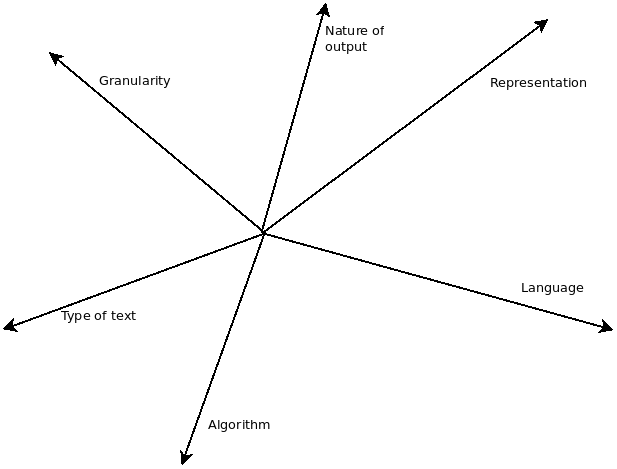
\includegraphics[width=\textwidth]{SentimentAnalysisProblemClassification.png}
\end{figure}

\clearpage

\begin{enumerate}
 \item Granularity of Text
 \item Type of text
 \item Algorithm
 \item Language
 \item Representation
 \item Nature of Output
\end{enumerate}

All these features collectively characterize a particular problem in SA. A change in even one of the features will change the
problem.

\section{Challenges}
\textit{SA} is a complex problem and has many challenges involved. In this section, an attempt is made to discuss some of the most notorious
difficulties in \textit{SA}. 

\subsection{Unstructured Text}
Text in micro-blogs, tweets, comments, and messages is unstructured. Most of the research in \textit{NLP} and many \textit{NLP} tools focus on structured
data. To adapt and use these tools for \textit{SA} is a big challenge. 

\subsection{Sarcasm}
Nowadays, many tweets and comments are sarcastic. Let us see an example on tweet, \textit{"Great! I ate too many chocolates and
gained lot of weight :)"}. This sentence will be marked as positive by almost any classifier. But, we can clearly see that this is
not a positive statement. Correctly, classifying such sentences will require context knowledge.

\subsection{Thwarting}
In a thwarted expression, the sentences which contradict the overall polarity of the document are in majority. An example is,
\textit{"The guy is a chronic drinker, he smokes weed, has drugs but is a good guy"}. The aim of thwarted expressions is to 
mislead the classifier. Detecting thwarted expressions is a very important difficulty.

\section{Applications of Sentiment Analysis}

We list some of the most important applications of \textit{SA}.

\begin{enumerate}
 \item	Classification of Tweets
 \item	Classification of Movie Reviews
 \item	Classification of Product Reviews
 \item	Analyzing market trends
 \item  Sentiment Aware Information Retrieval
 \item 	Removing subjective sentences to improve IR performance
\end{enumerate}

%----------------------------------------------------------------------------------------

\par
As we have discussed earlier, \textit{SA} is mainly a classification task. It can be thought of as a subset of a another important classification
task called \textit{Text classification}. Various approaches have been used to solve this problem. Most of them are machine learning 
based. This chapter takes a look at basic machine learning and some models in brief. Later on, combination of these models with other
techniques which take into consideration the various aspects of the \textit{text} are considered.

\section*{Approaches to Sentiment Analysis}

\section{Machine Learning}

\par

This section aims not to explain all the intricacies associated with machine learning but to provide a brief outline
which suffices for understanding future concepts. Machine learning by definition is learning from data. We have a mathematical
model, parameters of which have to be estimated from the data. By doing this we fit the model to the data provided. 
These parameters which have been \textit{learned} from the data can be said to completely define the model. Now this 
\textit{learned} model can be used for prediction or classification. In the case of \textit{SA}, \textit{Machine Learning} is used for classification
of \textit{text} as either positive, negative or neutral.

\par
The data available to us can be both labeled and unlabeled. By labeling we mean that the for an instance of the input we know
its class. Data labeling can also be called annotation. Labeled data is called annotated data. Depending upon the extent to which
the training data is labeled, we can classify the \textit{ML} techniques as follows.

\subsection{Supervised}
In this case, all the training data is a labeled. Majority of ML based techniques have this requirement that the data should be
completely labeled. The accuracy of the system decreases if the data is very small in size. This is called data sparsity problem.
They tend to over-fit if the data size is small.
\subsection{Unsupervised}
Here, the data is completely unlabeled. As opposed to supervised techniques, they do not suffer from data sparsity problem as 
the input in unlabeled.
\subsection{Semi-supervised}\label{subsection:semisupervised}
In this we have a mixture of both labeled and unlabeled data. Using the labeled data we try to annotate the unlabeled data. 
This technique is very useful if we have very sparse data.

\section{Feature Vector}
\par
Feature vector can be thought of as a way to represent the input. Some important aspects of the input are considered and used 
to represent it in the form of a vector of values. These values contain some important information which aids the classification
algorithm. 

\section{Models used for classification}
\par 
When we say we learn from the data, we actually train the model to do so. There are broadly two ways to do this. One is in a 
generative way and the other is discriminative. What do we actually mean by this? We want to infer the class of a \textit{text}.

\par
Let \textit{x} represent the input \textit{text}. We want to determine the class \textit{y} given the input \textit{i.e}, we are interested
in modeling \(p(y\mid x)\). There are three ways to do this.

\subsection{Generative Models}

\par 
One way is to model p(x, y) directly. Once we do that, we can obtain \(p(y \mid x)\) by simply conditioning on x. And we can then use decision 
theory to determine class membership \textit{i.e}, we can use loss matrix, \textit{etc}. to determine which class the point belongs to (such an assignment 
would minimize the expected loss). We can learn p(y), the prior class probabilities from the data. We can also learn \(p(x\mid y)\) from
the data using say maximum likelihood estimation (or we can Bayes estimator, if you will). Once you have p(y) and \(p(x\mid y)\), p(x, y) is 
not difficult to find out.

Bayes' rule is given as follows,

\begin{equation}
  p(y\mid x) = \frac{p(x\mid y)p(y)}{p(x)}
\end{equation}

\subsection{Discriminative Models}
Instead of modeling p(x, y), we can directly model \(p(y\mid x)\), for \textit{e.g}, in logistic regression \(p(y\mid x)\) is assumed to be of the form, 

\begin{equation}
  p(y\mid x) = \frac{1}{1 + \mathrm{e}^{(-\Sigma(wi.xi))}}
\end{equation}

All we have to do in such a case is to learn weights that would minimize the squared loss.

\par
There is a very easy technique to tell whether a model is generative or discriminative. If we can a generate new training data
using the model then it is certainly generative. In the case of generative models, the distribution \(p(x\mid y)\) is a model 
which fits the training data so it can be used to generate new data. In the case of discriminative models, this is not the case.

\subsection{Encoding a function}
We find a function f(.) that directly maps x to a class. The best example of this is decision trees. 

\section{Models}

Here, we explain the various machine learning models used.

\subsection{Naive Bayes classifier}
\par
Naive Bayes classifier is a generative classifier with strong independence assumptions. This means that all the features in feature
vector are independent of each other given the class. Despite of this very naive assumption, it gives surprisingly good results.
The parameters are estimated using the method of maximum likelihood.

Suppose we want to determine value of the class variable \textit{C} of the given input consisting of feature variables \textit{F_1,\dots,F_n}, 
it can be expressed as a conditioned probability \(p(C\mid F_1,\dots,F_n)\) using the Bayes' theorem,

\begin{equation}  
p(C\mid F_1,\dots,F_n) = \frac{p(C)p(F_1,\dots,F_n\mid C)}{p(F_1,\dots,F_n)}
\end{equation}

To use this equation for classification of a given input \textit{x} which is represented by a feature vector \textit{(F_1=f_1,\dots,F_n=f_n)},
the following equation is used,

\begin{equation}
class(f_1,\dots,f_n) = \arg\max_c p(C=c) \prod_{i=1}^{n} p(F_i = f_i \mid C=c) 
\end{equation}

\par
The main advantage of Naive Bayes is that it gives remarkably high accuracy for relatively small data sets because of the independence
assumption. 

\subsection{Maximum Entropy}
\par
Maximum Entropy more commonly known as \textit{MaxEnt} is a discriminative classifier. As it is a discriminative classifier, here we find out 
the conditional distribution of the class variable. The basic principle underlying maximum entropy is that without external knowledge
one should prefer distributions which are uniform and have maximum entropy. Using the training data, constraints on the distribution 
are derived which can be used to infer where the distribution should be minimally non-uniform. These constraints represent the expected
values of the features \citep*{nigam1999using}. In Text classification, \textit{MaxEnt} estimates the conditional distribution of the class label
given the \textit{text}. Representation of the \textit{text} is mostly in terms of word count features or word presence features.

 
Let \textit{f} be the features that link the observation \textit{x} to the class \textit{c}. A feature in this case is a function denoted
by \textit{f_i(x,c)} with a bounded real value. Also, let \textit{X} denote the collection of \textit{texts}. The aim of \textit{MaxEnt} is to
restrict the model distribution to have the same expected value for each such feature as is seen in the training data \textit{X}. 
This means that the learned conditional distribution \(p(c \mid x)\) must satisfy the following property, 

\begin{equation}\label{eqn:property}
 \frac{1}{|X|} \sum_{x \in X} f_i(x, c(x)) = \sum_x p(x) \sum_c p(c \mid x)f_i(x,c)
\end{equation}

equation ~\ref{eqn:property} reduces to the following form as we are not interested in modeling the collection \textit{X} here.

\begin{equation}\label{eqn:newproperty}
 \frac{1}{|X|} \sum_{x \in X} f_i(x, c(x)) = \frac{1}{|X|} \sum_{x \in X} \sum_c p(c \mid x)f_i(x,c)
\end{equation}

Feature identification is very important in this case. Using the training data, expected value of features is used as a constraint
for the model distribution. A class label for which most of these constraints are satisfied is the class of the given input \textit{x}.

\subsection{SVM}
A basic \textit{SVM} is a non-probabilistic binary linear classifier which given an input data predicts which of the two possible classes
forms the output.

\section{Usage in SA}

We have covered lot of basics to easily understand some of the techniques used for SA. We start with a basic bag of words model 
and then move on to more advanced techniques which incorporate the attributes of \textit{text}. Discourse based technique is 
discussed followed by a technique which makes use of minimum cut of a graph. These are followed by an unsupervised method which
makes use of a search engine called \textit{Alta Vista} to determine the semantic orientation of the \textit{text}. The last method
we discuss is a semi-supervised method which aims to perform ternary classification of sentences. 

\subsection{Bag of Words}

In a Bag of Words model, the feature vector is just a unigram model which is used to represent the presence or absence of a word.
Let us consider an example sentence, \textit{"I hate to play football"} and suppose the vocabulary \textit{V} is \(\left\{I, You, like, 
hate, to, for, play, dance, football, cricket\right\}\). In this case,  the feature vector will be \textit{(1,0,0,1,1,0,1,0,1,0)}.
We can see that here every word is a feature. In addition, it makes use of list of positive and negative words. If a word is positive
then the value corresponding to that feature is +1 and if it is negative the value is -1. Thus for the example is our case, the 
feature vector after making use of this dictionary becomes \textit{(1,0,0,-1,1,0,1,0,1,0)}. This feature vector is nothing but
a representation of the input. If sum of all the values is positive then the sentence has positive polarity and if it is less than
zero then it has negative polarity. For our example, it turns out that the sentence is negative. The accuracy of such a system though 
is not very good, around 65 \%.

On the other hand, If this input is fed to a default classifier like \textit{NB}, \textit{SVM} or \textit{MaxEnt} then it is shown to have a considerable increase
in accuracy\citep*{go2009twitter}. In \citep*{go2009twitter}, they conducted various experiments and got the results as shown in table
\ref{table:classifierAccuracy}

\begin{table}
 \caption{Classifier Accuracy}
 \begin{center}
 \begin{tabular}{| c | c | c | c | c | }
  \hline
  Features 		& Keywords & Naive Bayes & MaxEnt & SVM \\ \hline
  Unigram  		& 65.2 & 81.3 & 80.5 & 82.2 \\ \hline
  Bigram 		& N/A & 81.6 & 79.1 &78.8 \\ \hline
  Unigram + Bigram 	& N/A & 82.7 & 83.0 & 81.6 \\ \hline
  Unigram + POS 	& N/A & 79.9 & 79.9 & 81.9 \\
  \hline
 \end{tabular}
 \end{center}
 \label{table:classifierAccuracy}
\end{table}

\subsection{Adding Discourse information}

\par
Discourse elements have a sentiment changing impact on sentences. Let us consider an example,

\begin{center} \textit{"The screenplay was good but I didn't like the movie"}\end{center}

\par
Feature vectors discussed in the previous section won't be able to encode the information in such sentences. Using Bag of Words 
model can result in classification to a completely opposite polarity. To detect the polarity of such a sentence, detection of 
discourse elements and determining their effect is very important. Many approaches for this are present but all of them are for 
structured data and on most of the micro-blogging sites, the content is unstructured. Unstructured data is the main reason that 
many sentiment analysis tools make use of bag-of-words model. 


\par
To solve this problem, it is important to categorize the various types of discourse relations and find out the semantic operators 
which play a major role. In \citep*{mukherjeesentiment}, discourse relations have been categorized and many examples have been given to emphasize on 
some specific relation. Also, the semantic operations influencing the polarity have been explained. The algorithm then takes
into consideration all these attributes to create a feature vector. A weight is assigned to each valence shifter taking into 
consideration its position w.r.t the discourse element. Also, the polarity/sense of a particular word is flipped depending upon 
its position. It also makes an attempt to take into account the impact of  modals, which should lower the weight in some cases. 
The feature vector thus consists of weight, polarity, flipping and modality values for each word in the sentence. Words having 
zero weight have do not affect the polarity in any way and are thus ignored while calculation. The Feature vector thus created can be used for calculation the sentiment behind the sentence.
Two methods have been used, one is Lexicon based classification and the other is \textit{SVM} classification. In the \textit{SVM} classification, 
words with the same root are represented with a single vector. Also, special handling of \textit{emoticons} is present. \textit{WSD} is also used
to determine the exact sense of each word. The results show that this algorithm outperforms all the methods by a margin which has
statistically significant. Also, since this is lightweight and extends the baseline bag-of-words model, the performance of the 
system is very good. 

\subsection{Influence of Objective sentences on Classification}\label{section:subanalysis}

In \citep*{pang2004sentimental}, they have attempted to classify movie reviews as positive or negative. In this case the granularity
of the \textit{text} is a \textit{document}. Movie reviews often contain description of the plot. This description might contain
polar sentences but they have no relation whatsoever with the review about the movie. These sentences don't help in describing
about how good or bad the movie is. Consider the following example sentence from the review of a recent movie,

\textit{"The action follows Jean Valjean, a former convict, as he flees Javert, a fanatical police officer, through
a version of 19th-century France peopled with various grotesques, victims and tarnished saints."}

As we can see this sentence has a number of words with negative polarity. This will be classified as a negative sentence which 
might lead to the review as a whole being classified as negative. But, we know that this sentence is from the description of the 
plot and is not an opinion/review about the movie. To solve this problem, we need to identify which sentences are objective and discard them.
Subjective sentences in this scenario mean those sentences which are meant to describe the plot or contain some factual information.

The approach followed in \citep*{pang2004sentimental} has three steps,

\begin{enumerate}
 \item 	Label the sentences in the document subjective or objective
 \item The objective sentences are discarded. This extraction is based on minimum cut formulation which integrates inter-sentence contextual
information with Bag of Words model
 \item A standard machine learning approach is applied to the extract for polarity classification
\end{enumerate}

\subsubsection*{Subjectivity Detection}

This is the first step in their approach. They try to identify subjective sentences. For this, they have made use of cut-based
classification. Also, coherence of sentences is also taken into consideration. Coherence means that subjectivity status of two 
sentences close to each other may be same.

\textit{"I really loved the screenplay of this one. Award Winning Directors are often good at making such movies"}

As we can see from this example, two coherent sentences should ideally be classified under the same class.

\subsubsection*{Cut-based classification}

Let \(x_1,\dots,x_n\) be the sentences in the \textit{document}. Also, let \(C_1,\dots,C_k\) be the classes into which the sentences are to be classified.
There are two important sources of information which can aid the classification. 

\begin{enumerate}
 \item Individual scores: \(ind_i(x_i)\) - Preference of each \(x_i\) for being in class \(C_j\)
 \item Association scores: \(asso(x_i , x_j)\) - Estimate of how important it is that \(x_i\) and \(x_j\) are in the same class
\end{enumerate}

So, in the cut based classification penalizes if tightly associated items are put in different classes. So, taking into consideration,
the objective is to minimize the cost given below.

\begin{equation}
 \sum_{x\in C_1} ind_2(x) + \sum_{x\in C_2} ind_1(x) + \sum_{x_i \in C_1, x_k \in C_2} assoc(x_i,x_k)
\end{equation}

Now, we can see that this problem in intractable as there are 2^n possible partitions of x_i's. This minimization problem can be solved by
building an undirected graph \(G\) with vertexes \({ v_1, v_2 , v_3 ,\dots, v_n , s, t }\) . The last two are source and the sink and represent the two classes

The graph consists of following edges

\begin{enumerate}
  \item \(n\) edges \((s, v_i )\) with weight \(ind_1 (x_i )\)
  \item \(n\) edges \((t, v_i )\) with weight \(ind_2(x_i)\)
%   \item \( n \choose 2 \) edges \((v_i , v_k )\) each with weight \(assoc(x_i , x_k )\)
\end{enumerate}

A cut \((S, T)\) of \(G\) is a partition of its nodes into sets \(S = {s} \cup S\) and \(T = {t} \cup T\) where \(S\) does not contain 
\(s\) and \(T\) does not contain \(s\). Its cost \(cost(S, T )\) is the sum of the weights of all edges crossing from \(S\) to \(T\). 
A minimum cut of \(G\) is one of minimum cost.

\subsubsection*{Polarity classification}

Using the cut-based classification, we get the subjective sentences in the movie review. This extract is the fed to default polarity classifiers
which in this case are \textit{NB} and \textit{SVM}. The feature vector used for them is unigram based. 

\subsubsection*{Significance}

A cleaner document can be obtained by extracting only the subjective information. The accuracy of the polarity classification
improves as they don't get irrelevant data.The performance of the system will improve as it has less text to work on.

\subsection{Unsupervised semantic orientation}

A completely unsupervised approach to SA has been used in \citep*{turney2002thumbs}. It is aimed for classification of reviews about
products, automobiles, review, \textit{etc}. The approach used has three steps.

\begin{enumerate}
 \item Find phrases in the review containing adjectives and adverbs
 \item Find semantic orientation of such phrases
 \item Take avg of semantic orientation. If it is positive then \textit{Thumbs up} else \textit{Thumbs down}
\end{enumerate}

\subsubsection*{Step 1}

Extract phrases containing adjectives or adverbs. Adjectives are good indicators of subjectivity. Adjectives in isolation have 
insufficient context to determine semantic orientation. \textit{e.g}, \textit{“unpredictable”} when applied to \textit{“steering”} in a car 
review has negative semantic orientation. On the other hand \textit{“unpredictable plot”} in a movie review has positive orientation.

Therefore the algorithm uses 2 consecutive words where one is adjective/adverb and the other provides context.

\subsubsection*{Step 2}

\subsubsection*{Point-wise Mutual Information (PMI)}
Point-wise Mutual Information between two words word1 and word2 is defined as

\begin{equation}
PMI(word_1,word_2) = log_2 \Bigg[ \frac{p(word_1 \wedge word_2)}{p(word_1)p(word_2} \Bigg]
\end{equation}

where \(p(word_1 \wedge word_2 )\) is the probability that \(word_1\) and \(word_2\) co-occur.

\subsubsection*{Semantic Orientation}

Semantic orientation of a phrase is given by,

\begin{equation}
\label{eqn:SO}
SO(phrase) = PMI(phrase, excellent) - PMI(phrase,poor)
\end{equation}
  
The \textit{PMI} are estimated by issuing queries to a search engine which explains the \textit{IR} in \textit{PMI-IR}. It notes 
the number of hits to calculate the probability values. The search engine used in this case was \textit{AltaVista}.

After some algebraic simplifications and using the fact that \(p(phrase,excellent) = \textit{hits(phrase NEAR excellent)} \), 
equation \ref{eqn:SO} reduces to the following form:

\begin{equation}
SO(phrase) = log_2 \Bigg[ \frac{\textit{hits(phrase NEAR excellent)hits(poor)}}{\textit{hits(phrase NEAR poor)hits(excellent)}} \Bigg]
\end{equation}

Here, \textit{hits(query)} stands for the number of hits returned by the query.

\subsubsection*{Step 3}

In this step, average of the semantic orientations of all the phrases is taken.

\begin{itemize}
  \item If the avg is positive then Thumbs Up.
  \item If the avg is negative then Thumbs Down.
\end{itemize}

\subsubsection*{Observations}

After experiments were conducted, following observations were made.

\begin{itemize}
 \item Movie Reviews are hard to classify because a good movie might contain unpleasant scenes. Description of such scenes might decrease the
	semantic orientation.
 \item Accuracy did not increase just by accounting for this bias using a constant value. Just as positive reviews have description of unpleasant scenes, negative reviews might
	contain description of pleasant scenes.

\end{itemize}

\subsubsection*{Limitations}

This approach has some limitations as can be seen from the architecture. 

\begin{itemize}
 \item Queries search engine to calculate semantic orientation of each phrase.
 \item Every phrase is given equal importance. There should be a weighted sum.
 \item The performance in case of movie reviews is not good because it does not take into account the fact that the whole is not
	necessarily a sum of parts as pointed out in section. \ref{section:subanalysis}
\end{itemize}

\subsection{Semi-supervised}

A semi-supervised approach for detecting term orientation was used in \citep*{esuli2006determining}. 
In \citep*{esuli2006determining}, they have tried to perform a ternary classification of terms as objective, positive, or negative. 
The motivation behind this study is that in most works which determine the term orientation, it is assumed that we already know 
whether it a subjective term or not. So, we assume that a lexical resource of subjective/objective terms is available. This is not 
the case. 

Semi-supervised was discussed briefly in section \ref{subsection:semisupervised}. Semi-supervised can be depicted as shown in figure 2.1

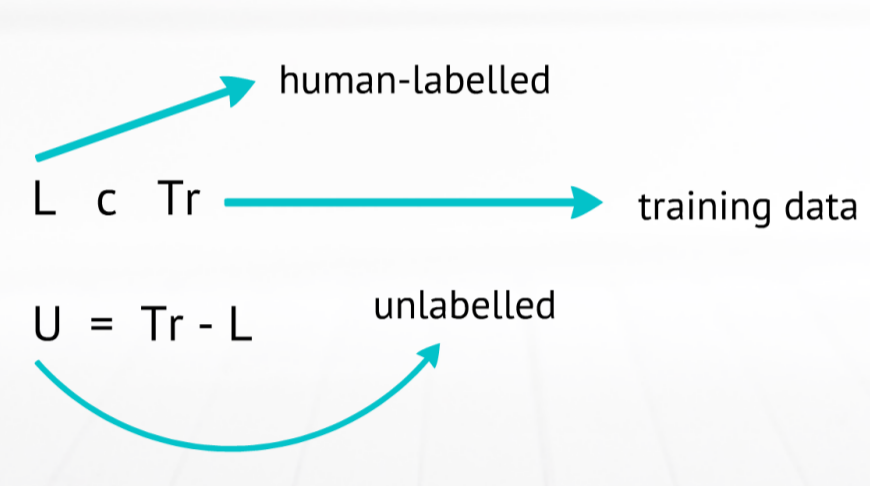
\includegraphics[width=\textwidth]{semisupervised}

\begin{center}
 Figure 2.1 Training Data in semi-supervised learning
\end{center}

 
The unlabeled data has to be labeled and it should also be used for training. The labeled usually is called as seed set.
In \citep*{esuli2006determining}, they have made used of synonymy-antonymy relations of the wordnet to create the training data. 

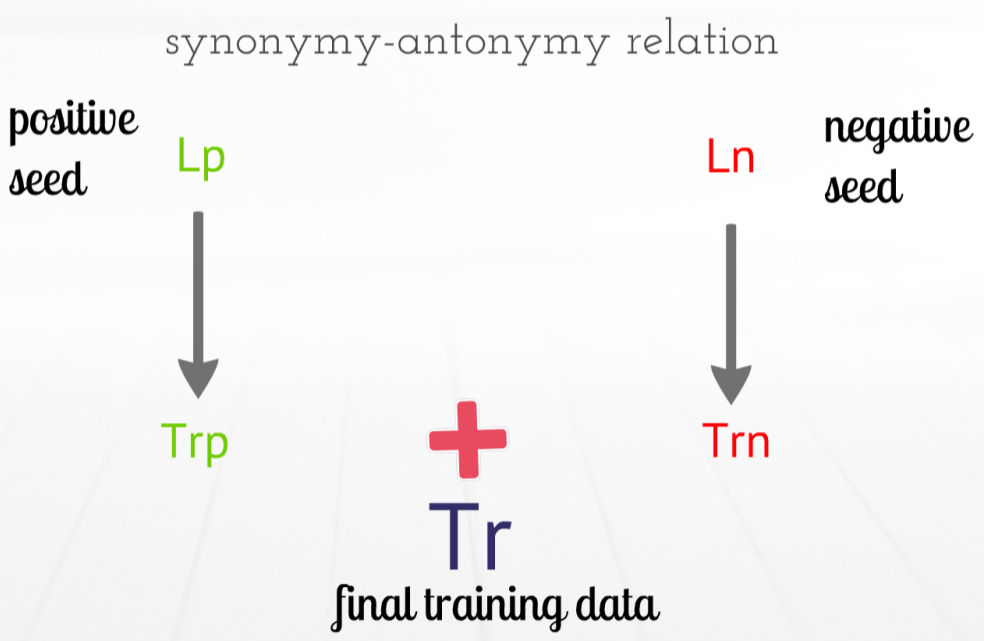
\includegraphics[width=\textwidth]{synonymyantonymyrelation}
\begin{center}
 Figure 2.2 Using synonymy-antonymy relation for labeling unlabeled data
\end{center}


As we can see, we start with very small seed sets in this case, each containing only one element. The exact procedure is shown in 
the figure 2.3.

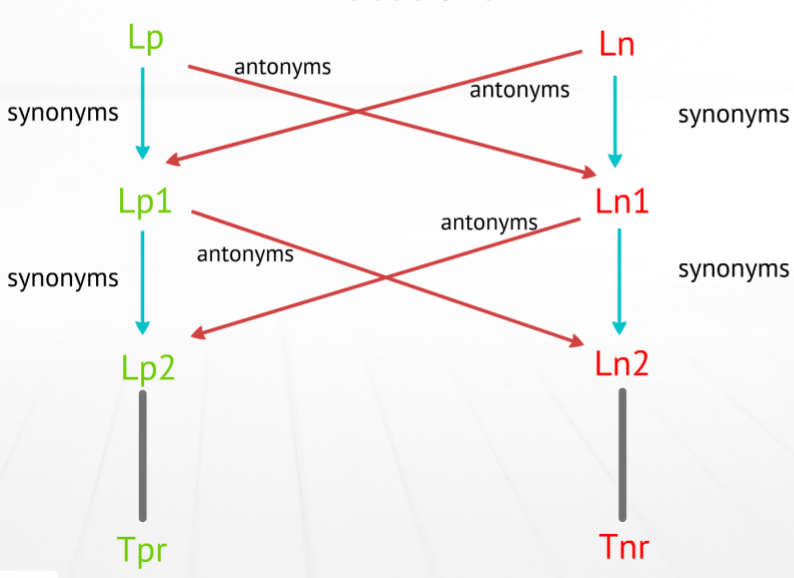
\includegraphics[width=\textwidth,height=0.6\textwidth]{procedure}
\begin{center}
 Figure 2.3 Procedure for labeling unlabeled data using synonymy-antonymy relation
\end{center}


\par
After getting all the training data, a textual representation for each term is generated by collating all the wordnet glosses
for that term. A cosine normalized \textit{TF-IDF} representation is used as the feature vector. The result obtained by the approaches used
in this paper were not that accurate and they show that algorithm used for term orientation when used for ternary classification
perform badly and need improvement.

\section*{SUMMARY}

In this chapter we introduced \textit{Sentiment Analysis}. The motivation behind this work was discussed. A psychological viewpoint of 
\textit{SA} was explained. A formal problem definition of sentiment analysis was given. This was followed by depicting the various 
dimensions of a problem in \textit{SA}. Prevalent challenges in sentiment analysis were discussed briefly and some major applications were
listed. Then we started with the basics of Machine Learning. Then we explained the various approaches and techniques used
in ML. We explained what is a feature vector. Moving forward, we tried to understand the different models used in ML. Works using
all these techniques were explained.

In the next chapter we will discuss information retrieval and the focus on corpus models, mainly \textit{LDA}.

\clearpage 
% Chapter 3

\chapter{Information Retrieval} % Main chapter title

\label{ir} % For referencing the chapter elsewhere, use \ref{Chapter3} 

\lhead{Chapter 3. \emph{Information Retrieval}} % This is for the header on each page - perhaps a shortened title

%----------------------------------------------------------------------------------------

\section{Information Retrieval}

\par 
In simple terms Information Retrieval is the process of retrieving information relevant to the need. As the web contains lot of
information, finding most relevant information is very difficult. A user usually requests information in the form of a query.
The retrieval engine then presents the user set of documents relevant to the user's query. As the web contains lot of noise, it
is difficult to fetch all the relevant documents. It should be noted that IR is not only concerned with the web as a resource of
information. Precision, Recall, and F-measure are the important performance measures of an IR system. They are defined as follows.

\subsection*{Precision}

\textit{Precision} is the fraction of documents that are relevant to the query

\begin{equation}
 Precision = \frac{|\{\textit{relevant documents}\} \cap \{\textit{retrieved documents}\}|}{|\{\textit{retrieved documents}\}|}
\end{equation}

\subsection*{Recall}

\textit{Recall} is the fraction of the documents that are relevant to the query that are successfully retrieved

\begin{equation}
 Recall = \frac{|\{\textit{relevant documents}\} \cap \{\textit{retrieved documents}\}|}{|\{\textit{relevant documents}\}|}
\end{equation}

\subsection*{F-measure}

\textit{F-measure} is the harmonic mean of \textit{Precision} and \textit{Recall}

\begin{equation}
 F = \frac{2.Precision.Recall}{(Precision+Recall)}
\end{equation}

\par

Text indexing, relevance ranking, similarity search and corpus modeling are amongst the most important approaches used for 
\textit{IR}. In the next section, we will show how sentiment analysis for sentiment-aware IR.

\section{Sentiment Aware IR}

In this section we will be discussing about two systems implemented to use \textit{sentiment analysis} in \textit{information retrieval}.

\begin{enumerate}
 \item Indexing followed by Sentiment Analysis
 \item Encoding sentiment in the Index
\end{enumerate}

As can be seen by the brief description, the first one uses a staged approach and the second one is a one-stage process but involves
some heavy preprocessing to predict the sentiment of the \textit{text}. These approaches are very simple and aren't novel.
These systems have merely been discussed to show the novelty of some future work. \textit{Lucene} \citep*{apachelucene} was used for indexing
in both these systems.

\subsection{Indexing followed by Sentiment Analysis}

\subsection*{Architecture}

\begin{enumerate}
 \item Lucene
  \par It has a variety of features to perform indexing from basic to very advanced. 
 \item Query Processor
  \par This is also a part of of lucene. The objective content of the query is processed by this component
 \item Sentiment Analyzer
  \par Sentiwordnet \citep*{sentiwordnet} was used to calculate the score of each word. The sentiment for a sentence was a sum of sentiment scores
  for each word. Sentiment of the whole document was a sum of sentiments for all the sentences. 
\end{enumerate}

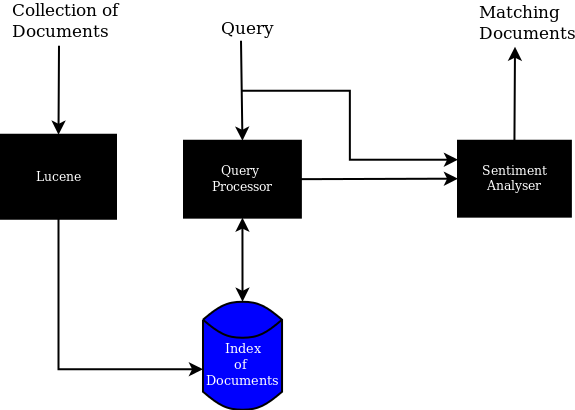
\includegraphics[width=\textwidth]{IndexingFollowedBySentimentAnalysis}
\begin{center}
 Figure 3.1 Indexing Followed by Sentiment Analysis
\end{center}

\subsection{Encoding sentiment in the Index}

\subsection*{Architecture}

\begin{enumerate}
 \item Lucene + Sentiment Analyzer
  \par It has a variety of features to perform indexing from basic to very advanced. In this case, sentiment analysis was combined with
  indexing. One more field, \textit{sentiment} was added to the index. This value was inferred using the sentiment analyzer. 
 \item Query Processor
  \par In this case, both the subjective and objective content of the query was processed. The documents were fetched based on the objective
  content of the query. Then, depending on the value of the \textit{sentiment} field, these fetched documents were filtered and presented
  to the user.
\end{enumerate}

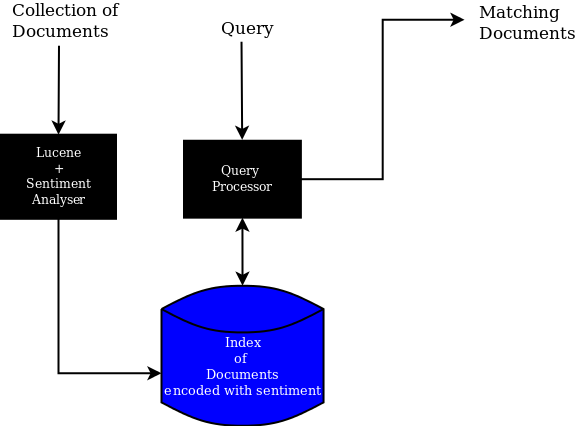
\includegraphics[width=\textwidth]{SentimentEncodedInIndex}
\begin{center}
 Figure 3.2 Encoding Sentiment in Index
\end{center}

Both these systems can be very useful. But as we can see the first one incurs lot of processing overhead and the second one has lot of 
preprocessing overhead. Also, both follow a procedural approach. A more novel approach will be two combine sentiment and topic to create 
a model which we can fit to our training data and then infer the resemblance of a new document to existing ones.

In this chapter we will focus on corpus modeling as in most works combining \textit{SA} and \textit{IR}, corpus modeling has been used. 
This draws directly from the Language Modeling approach used in many \textit{NLP} systems. In the next section we focus on the different
types of Corpus models. One effort towards using language modeling for \textit{IR} was made in \citep*{ponte1998language}

\section{Corpus Models}

Corpus models are the probabilistic language models using which we can perform retrieval. In this section, we will have a look 
at multivariate binary model, \textit{poisson} model, \textit{multinomial} model, \textit{DCM}, \textit{dirichlet} smoothed models, and \textit{LDA}. 
One advantage of using models to perform text retrieval is that the models can be refined independent of the retrieval algorithm. 

\subsection{Multivariate Binary Model}

A document in this model is represented as a bit vector where the presence or absence of a word in the vocabulary is represented 
by a bit. The probability of a document \(x\) is given by,

\begin{align}\label{eqn:multivariatebinary}
Pr(x \mid \phi )	& = \prod_{w \in W} {\phi_w}^{x_w}{(1-\phi_w)}^{1-x_w}\\
			& = \prod_{w \in W} \phi_w \prod_{w \in W, w \notin x} (1-\phi_w)
\end{align}

\(w\) in equation \ref{eqn:multivariatebinary} is a word in vocabulary \(W\). This model does not work well for short documents
because in that case \(|W| \gg |x|\). Also, the product  make strong independence assumptions leading to the underestimation of
\(Pr(x \mid \phi)\).

\subsection{Poisson Model}

In the previous model, word counts were not taken into consideration. For this model, the document will be represented by a
vector of word counts. Every word \(w\) has a parameter \(\mu_w\) associated with it. In this model, it is assumed that word
counts are random variables \(X_w\) that follow \textit{poisson} distributions with means \(\mu_w\) as follows:

\begin{equation}
 Pr(\textit{X_w = z}) = \frac{e^{-\mu_w}{\mu_w}^z}{z!}, \textit{z = 0,1,2,\dots}
\end{equation}

The probability of invoking the Poisson document generator and getting a count vector x is given as:

\begin{align}
 Pr(x \mid \mu)		& = \prod_{\textit{all w}} Pr(\textit{X_w = x_w}) \\
			& = \prod_{\textit{all w}} \frac{e^{-\mu_w}{\mu_w}^{x_w}}{x_w!} \\
			& = \textit exp(-\sum_{all w} \mu_w) \prod_{w \in x} \frac{{\mu_w}^{x_w}}{x_w!}
\end{align}

\subsection{Multinomial Model}

In the previous two models, we were not able to model the document length. In this model, we can take that aspect of the document
into consideration. Let \(L\) be the random variable for the document length. The length of the document in sampled from the 
distribution of this variable. For each word \(w\) in the vocabulary \(W\), a probability \(\theta_w\) is present. Let \(x_w\)
denote the count of word \(w\) and \(l_x\) denotes length of the document. 

The probability of the document with length \(l_x\) is given by:

\begin{align}
 Pr(l_x,\{ x_w \})	& = Pr(L=l_x)Pr(\{x_w\}|l_x,\theta) \\
			& = Pr(L=l_x) {{l_x} \choose {\{x_w\}}} \prod_{w \in x} {\theta_x}^{x_w} \\
			& = Pr(L=l_x) l_x! \prod_{w \in x} \frac{(\theta_x^{x_w}}{x_w!}
\end{align}

The drawback with the models discussed so far is that do not handle unknown words. If the document contains a word \(w\) which
is not in the vocabulary \(W\) then it's probability will be zero. The models we see next overcome this drawback. They also
take into account the word \textit{burstiness} which means that when a word appears once in a document, it tends to appear more. 

\subsection{Dirichlet distribution model}

In this model too the document is represented as a vector of word counts. The problem with multinomial model is that it fails to 
account for word \textit{burstiness}. The nature of data according to \textit{Zipf's} law follows a model of the form \({data}^{parameter}\) but in
case of multinomial it is \({parameter}^{data}\). It is this intuition that lead to look for new models for representing data.

Dirichlet distribution is a probability density function over distributions given as

\begin{equation}\label{eqn:dirichlet}
 p(\theta \mid \alpha) = \frac{\Gamma \Big( \sum_{w=1}^W \alpha_w \Big)}{\prod_{w=1}^W \Gamma (\alpha_w)} \prod_{w=1}^W {\theta_w}^{\alpha_w - 1}
\end{equation}

Equation \ref{eqn:dirichlet} can be written exponential family form as

\begin{equation}
 logp(\theta \mid \alpha) = \sum_{w=1}^W (\alpha_w - 1) log \theta_w + log \Gamma (\sum_{w=1}^W \alpha_w) - \sum_{w=1}^W log\Gamma(\alpha_w)
\end{equation}

In this model, the representation of the document is in terms of a probability vector. 

Documents being sparse in nature \textit{i.e}, each document contains only a small subset of the vocabulary which might make the probability
zero. Smoothing can be used in this case. 

\subsection{DCM (Dirichlet Compound Multinomial Model)}

The problem with using smoothing in \textit{DCM} is that over-smoothing is done. In this case all the rare words have the same probability
of appearing in all the classes. Since, rare words are the main discriminators in classification, this model is not suitable for
classification \citep*{madsen2005modeling}. A hierarchical model can solve this problem. \textit{DCM} is one such model. It was introduced in \citep*{madsen2005modeling}.

To generate a document using the \textit{DCM}, a sample is first drawn from the Dirichlet to get a multinomial distribution, then words are
iteratively drawn for the document based on the multinomial distribution. \textit{DCM} can be thought of as a bag-of-bag-of-words-model.
\citep*{madsen2005modeling}


The probability of a document \(x\) is given by:

\begin{equation}
 p(x \mid \alpha) = \int_\theta p(x \mid \theta ) p(\theta \mid \alpha) \mathrm{d}x 
\end{equation}

\subsection{Latent Dirichlet Allocation}

All the models discussed previously were for a single topic. We now consider one multi-topic model, \textit{LDA}. It was introduced in 
\citep*{blei2003latent}. Latent Dirichlet allocation is a way of automatically discovering topics that documents contain. 

In more detail, \textit{LDA} represents documents as mixtures of topics that spit out words with certain probabilities. It assumes that 
documents are produced in the following fashion: 

\begin{itemize}

\item When writing each document, you decide on the number of words N the document will have.

\item Choose a topic mixture for the document using dirichlet hypergenerator.

\item Generate each word in the document by:
  
  \begin{enumerate}
  
  \item First picking a topic using the multinomial distribution generated from the dirichlet hypergenerator.
  
  \item Then using the topic to generate the word itself.

  \end{enumerate}

\end{itemize}

Assuming this generative model for a collection of documents, LDA then tries to backtrack from the documents to find a set of 
topics that are likely to have generated the collection. A detailed discussion of LDA can be found in the next section.

\section{Latent Dirichlet Allocation}

\par

\textit{Latent Dirichlet Allocation} is a probabilistic generative model. It is completely unsupervised in nature. The main goal of 
\textit{LDA} is to do \textit{Latent Semantic Analysis} (\textit{LSA}). \textit{LSA} aims to find the latent structure of topics or 
concepts within a \textit{text}. \citep*{heinrich2005parameter} gives a very thorough explanation for \textit{LDA} and the inference 
method used. Most of the content in this chapter has been borrowed from \citep*{heinrich2005parameter}.

\subsection{Bayesian Network for LDA}

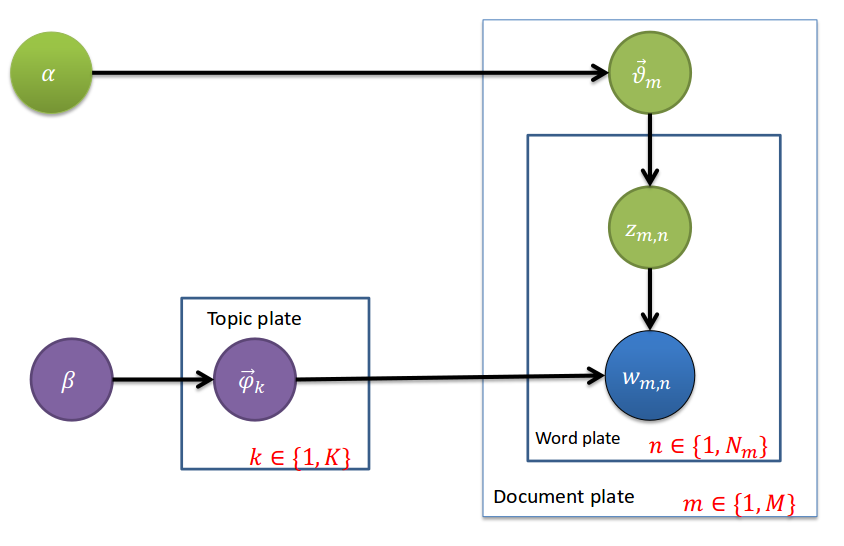
\includegraphics[width=\textwidth]{lda/lda.png} 
\begin{center}
 Figure 3.1 Bayesian Network for Latent Dirichlet Allocation
\end{center}

\textit{Bayesian Network} is a \textit{directed acyclic graph} (\textit{DAG}) where nodes correspond to random variables and edges correspond
to conditional probability distributions. The replication of a node is represented by a \textit{plate}. This is to account for multiple
values or mixture components.

\subsection{Generative Model for LDA}

The generative process for \textit{LDA} is as follows \(\colon\)

\begin{alltt}
\(\Box\) Topic Plate \(\colon\)
\textbf{for} all topics \( k \in [1,K] \) \textbf{do}
  sample mixture components \( \vec{\psi_k} \sim Dir(\vec{\beta}) \)
\textbf{end for}
\(\Box\) Document Plate \(\colon\)
\textbf{for} all documents \( m \in [1,M] \) \textbf{do}
  sample mixture proportion \( \vec{\vartheta_m} \sim Dir(\vec{\alpha}) \)
  sample document length \( N_m \sim Poiss(\xi)\)
  \(\Box\) Word Plate \(\colon\)
  \textbf{for} all words \( n \in [1,N_m] \) in document m \textbf{do}
    sample topic index \( z_{m,n} \sim Mult(\vec{\vartheta}_m) \)
    sample term for word \( w_{m,n} \sim Mult(\vec{\psi}_{z_{m,n}}) \)
  \textbf{end for}
\textbf{end for}
\end{alltt}

\subsection{Likelihoods}

Probability that a particular word \(w_{m,n}\) instantiates a particular term \(t\) given the \textit{LDA} parameters is,

\begin{equation}\label{eqn:likelihood}
 p(w_{m,n}=t|\vec{\vartheta}_m,\underline{\phi}) = \sum_{k=1}^{K} p(w_{m,n}=t|\vec{\psi}_k)p(z_{m,n}=k|\vec{\vartheta}_m)
\end{equation}

\eref{eqn:likelihood} corresponds to one iteration on the word plate of the bayesian network.

Joint distribution of all known and hidden variables given the hyperparameters is given by,

\begin{equation}
p(\vec{w}_m,\vec{z}_m,\vec{\vartheta}_m,\underline{\phi}|\vec{\alpha},\vec{\beta}) = 
\prod_{n=1}^{N_m} p(w_{m,n}|\vec{\psi}_{z_{m,n}})p(z_{m,n}|\vec{\vartheta}_m).p(\vec{\vartheta}_m|\vec{\alpha}).p(\underline{\phi}|\vec{\beta})
\end{equation}

Likelihood of one document is given by,

\begin{align}
p(\vec{w}_m|\vec{\alpha},\vec{\beta})		& = \iint p(\vec{\vartheta}_m|\vec{\alpha}).p(\underline{\phi}|\vec{\beta}).\prod_{n=1}^{N_m} \sum_{z_{m,n}} p(w_{m,n}|\vec{\psi}_{z_{m,n}})p(z_{m,n}|\vec{\vartheta}_m)d\underline{\phi}d\vec{\vartheta}_m \\                                  
						& = \iint p(\vec{\vartheta}_m|\vec{\alpha}).p(\underline{\phi}|\vec{\beta}).\prod_{n=1}^{N_m} p(w_{m,n}|\vec{\vartheta}_m,\underline{\phi}) d\underline{\phi}d\vec{\vartheta}_m
\end{align}

Likelihood of the whole corpus \(W = \{\vec{w}_m\}_{m=1}^{M}\) is given by,

\begin{equation}
p(W|\vec{\alpha},\vec{\beta}) = \prod_{m=1}^{M} p(\vec{w}_m|\vec{\alpha},\vec{\beta})
\end{equation}

Let us describe the quantities used in the model

\begin{alltt}
\(M\) number of documents to generate (const scalar).
\(K\) number of topics/mixture components (const scalar).
\(V\) number of terms \(t\) in vocabulary (const scalar).
\(\vec{\alpha}\) hyper-parameter on the mixing proportions (\(K-vector\) or scalar if symmetric).
\(\vec{\beta}\) hyper-parameter on the mixing components (\(K-vector\) or scalar if symmetric).
\(\vec{\vartheta}_m\) parameter notation for p(z|d=m), the topic mixture proportion for document \(m\). 
  One proportion for each document, \(\underline{\theta} = \{\vec{\vartheta}_m\} m=1 \cdots M (M \times K matrix)\).
\(\vec{\psi}_k\) parameter notation for p(t|z=k), the mixture component of topic \(k\). 
  One component for each topic, \(\underline{\phi} = \{\vec{\psi}_k\} k=1 \cdots K (K \times V matrix)\).
\(N_m\) document length (document-specific), here modeled with a Poisson distribution with 
  constant parameter \(xi\).
\(z_{m,n}\) mixture indicator that chooses the topic for the nth word in document m.
\(w_{m,n}\) term indicator for the nth word in document m.
\end{alltt}

\subsection{Inference via Gibbs Sampling}

The exact inference is intractable in case of \textit{LDA}. An approximate inference via \textit{Gibbs} sampling is used. 

\par
\textit{Gibbs} Sampling \citep*{walsh2004markov} is a special case of \textit{Markov-chain Monte Carlo}. \textit{MCMC} can emulate high dimensional probability
distributions, \(p(\vec{x})\) by the stationary distribution of a \textit{Markov chain}. Each sample is generated for each transition in 
the chain. This is done after a stationary state of the chain has been reached which happens after a so-called ``burn-in period'' which 
eliminates the effect of initialization parameters. In \textit{Gibbs} sampling, the dimensions \(x_i\) of the distribution are sampled
alternately one at a time, conditioned on the values of all other dimensions, denoted by \(\vec{x}_{ \neg i}\)

\subsubsection*{Bivariate Case of Gibbs Sampling}

\par
Consider a bivariate random variable \((x,y)\), and suppose we wish to compute the marginals, \(p(x)\) and \(p(y)\). The idea behind the
sampler is that it is easier to consider a sequence of distributions, \(p(x|y)\) and \(p(y|x)\) than obtaining the marginal by integration,
\(p(x) = \int p(x,y) dy\).

\textbf{Steps}

\begin{enumerate}
 \item Start with some initial value \(y_0\) for \(y\).
 \item Obtain \(x_0\) by generating a random variable from a conditional distribution, \(p(x|y=y_0)\).
 \item Use \(x_0\) to generate a new value of \(y_1\) drawing from a conditional distribution, \(p(y|x=x_0)\).
\end{enumerate}

The sampler proceeds as follows, 

\begin{enumerate}
 \item \(x_i \sim p(x|y=y_i)\)
 \item \(y_i \sim p(y|x=x_{i-1})\)
\end{enumerate}

Repeating this process \(k\) times generates a \textit{Gibbs} sequence of length \(k\), where a subset of points \((x_j,y_j)\) for 
\(1 \leq j \leq m < k\) are taken as simulated draws from the full joint distribution.

\subsubsection*{Multivariate Case}

The value of the \(k^{th}\) variable is drawn from the distribution, \(p(\theta^{(k)}|\Theta^{\neg k})\) where \(\Theta^{\neg k}\) denotes
a vector containing all the variables but \(k\). 

We draw from the distribution,

\(\theta_{i}^{(k)} \sim p(\theta^{(k)} | \theta^{(1)}=\theta_{i}^{(1)}, \cdots,\theta^{(k-1)}=\theta_{i}^{(k-1)},\theta^{(k+1)}=\theta_{i-1}^{(k+1)},\cdots,\theta^{(n)}=\theta_{i-1}^{(n)})\)

For example, if there are four variables, \((w,x,y,z)\), the sampler becomes

\begin{enumerate}
 \item \(w_i \sim p(w | x = x_{i-1}, y = y_{i-1}, z = z_{i-1})\)
 \item \(x_i \sim p(x | w = w_{i}, y = y_{i-1}, z = z_{i-1})\)
 \item \(y_i \sim p(y | w = w_{i}, x = x_{i}, z = z_{i-1})\)
 \item \(z_i \sim p(z | w = w_{i}, x = x_{i}, y = y_{i})\)
\end{enumerate}

\subsubsection*{Gibbs Sampling Algorithm}

To get a sample \(p(x)\),

\begin{enumerate}
 \item Choose dimension \(i\) (random or by permutation)
 \item Sample \(x_i\) from \(p(x_i|\vec{x}_{\neg i})\)
\end{enumerate}

\begin{equation}
 p(x_i|\vec{x}_{\neg i}) = \frac{p(\vec{x})}{p(\vec{x}_{\neg i})} where, \vec{x} = \{x_i,\vec{x}_{\neg i}\}
\end{equation}

\subsubsection*{Gibbs Sampling for Models with Hidden Variables}

For models containing hidden variable, \(\vec{z}\), their posterior given the evidence, \(p(\vec{z}|\vec{x})\) is a distribution commonly
wanted. 

The general formula of a \textit{Gibbs} sampler for such latent variable models becomes, 

\begin{equation}
 p(z_i|\vec{z}_{\neg i},\vec{x}) = \frac{p(\vec{z},\vec{x})}{p(\vec{z}_{\neg i},\vec{x})}
\end{equation}

\subsubsection*{LDA Gibbs Sampler}

Target of inference is the distribution, \(p(\vec{z}|\vec{w})\)

\begin{equation}
 p(\vec{z}|\vec{w}) = \frac{\vec{z},\vec{w}}{p(\vec{w})} = \frac{\prod_{i=1}^{W} p(z_i,w_i)}{\prod_{i=1}^{W} \sum_{k=1}^{K} p(z_i=k,w_i)}
\end{equation}

Full conditional, 

\begin{equation}\label{eqn:fullconditionalincomplete}
p(z_i|\vec{z}_{\neg i},\vec{w}) 
\end{equation}

is used to simulate \(p(\vec{z}|\vec{w})\)

This requires the joint distribution, 

\begin{equation}
p(\vec{w},\vec{z}|\vec{\alpha},\vec{\beta}) = p(\vec{w}|\vec{z},\vec{\beta})p(\vec{z}|\vec{\alpha})\label{eqn:wzgivenalphbetaincomplete}
\end{equation}

\subsubsection*{Calculation of \(p(\vec{w}|\vec{z},\vec{\beta})\)}

\(W\) words of the corpus are observed according to independent multinomial trials,

\begin{equation}
 p(\vec{w}|\vec{z},\underline{\phi}) = \prod_{i=1}^{W} p(w_i|z_i) = \prod_{i=1}^{W} \psi_{z_i,w_i}
\end{equation}

Splitting the product over words into product over topics and one over vocabulary,

\begin{equation}\label{eqn:wgivenpsi}
 p(\vec{w}|\vec{z},\underline{\phi}) = \prod_{k=1}^{K} \prod_{t=1}^{V} p(w_i=t|z_i=k) = \prod_{k=1}^{K} \prod_{t=1}^{V} \psi_{k,t}^{n_{k}^{t}}
\end{equation}

where, \(n_k^{(t)}\) denotes the number of times that the term \(t\) has been observed with topic \(k\).

Integrating \eref{eqn:wgivenpsi} over \(\underline{\phi}\) we get,

\begin{align}
  p(\vec{w}|\vec{z},\vec{\beta})	& = \int p(\vec{w}|\vec{z},\underline{\phi})p(\underline{\phi}|\vec{\beta})d\underline{\phi} \\
					& = \int \prod_{z=1}^{K} \frac{1}{\Delta(\vec{\beta})} \prod_{t=1}^{V} \psi_{z,t}^{n_{z}^{t}+\beta_t-1}d\vec{\phi}_z \\ 
					& = \prod_{z=1}^{K} \frac{\Delta(\vec{n}_z+\vec{\beta})}{\Delta(\vec{\beta})}, \vec{n}_z = \{n_{z}^{(t)}\}_{t=1 \cdots N}
					\label{eqn:wgivenbeta}
\end{align}

\subsubsection*{Calculation of \(p(\vec{z}|\vec{\alpha})\)}

\begin{align}
 p(\vec{z}|\underline{\theta})		& = \prod_{i=1}^{W} p(z_i|d_i) \\
					& = \prod_{m=1}^{M} \prod_{k=1}^{K} p(z_i=k|d_i=m) \\
					& = \prod_{m=1}^{M} \prod_{k=1}^{K} \vartheta_{m,k}^{n_m^{k}} \label{eqn:zgiventheta}
\end{align}

where, \(d_i\) refers to the document a word \(i\) belongs to and \(n_m^{(k)}\) refers to the number of times that topic \(k\) has been observed
with a word of document \(m\).

Integrating \eref{eqn:zgiventheta} over \(\underline{\theta}\) we get,

\begin{align}
 p(\vec{z}|\vec{\alpha})		& = \int p(\vec{z}|\underline{\theta})p(\underline{\theta}|\vec{\alpha})d\underline{\theta} \\
					& = \int \prod_{m=1}^{M} \frac{1}{\Delta(\vec{\alpha})} \prod_{k=1}^{K} \vartheta_{m,k}^{n_m^{k} + \alpha_k - 1} d\vec{\vartheta}_m \\
					& = \prod_{m=1}^{M} \frac{\Delta(\vec{n}_m+\vec{\alpha})}{\Delta(\vec{\alpha})}, \vec{n}_m = \{n_{m}^{(k)}\}_{k=1 \cdots K}
					\label{eqn:zgivenalpha}
\end{align}

Putting \eref{eqn:zgivenalpha} and \eref{eqn:wgivenbeta} into \eref{eqn:wzgivenalphbetaincomplete} we get,

\begin{equation}\label{eqn:jointdistribution}
p(\vec{z},\vec{w}|\vec{\alpha},\vec{\beta}) = \prod_{z=1}^{K} \frac{\Delta(\vec{n}_z+\vec{\beta})}{\Delta(\vec{\beta})} \prod_{m=1}^{M} \frac{\Delta(\vec{n}_m+\vec{\alpha})}{\Delta(\vec{\alpha})}
\end{equation}

\eref{eqn:jointdistribution} is the joint distribution. 

Now, the full conditional given in \eref{eqn:fullconditionalincomplete} can be expressed as,
 
\begin{align}
p(z_i=k|\vec{z}_{\neg i},\vec{w})	& = \frac{p(\vec{w},\vec{z})}{p(\vec{w},\vec{z}_{\neg i})} \\
					& = \frac{p(\vec{w}|\vec{z})p(\vec{z})}{p(\vec{w}|\vec{z}_{\neg i})p(\vec{z}_{\neg i})} \\
					& \propto \frac{\Delta(\vec{n}_z+\vec{\beta})}{\Delta(\vec{\beta})} . \frac{\Delta(\vec{n}_m+\vec{\alpha})}{\Delta(\vec{\alpha})} \\
					& \propto \frac{\Gamma(n_{k}^{(t)} + \beta_t)\Gamma(\sum_{t=1}^{V} n_{k,\neg i}^{(t)} + \beta_t)}{\Gamma(n_{k,\neg i}^{(t)} + \beta_t)\Gamma(\sum_{t=1}^{V} n_{k}^{(t)} + \beta_t)}.
						  \frac{\Gamma(n_{m}^{(k)} + \alpha_k)\Gamma(\sum_{k=1}^{K} n_{m,\neg i}^{(k)} + \beta_t)}{\Gamma(n_{m,\neg i}^{(k)} + \beta_t)\Gamma(\sum_{k=1}^{K} n_{m}^{(k)} + \beta_t)} \\
					& \propto \frac{n_{k,\neg i}^{(t)} + \beta_t}{\sum_{t=1}^{V}n_{k,\neg i}^{(t)} + \beta_t}.
						  \frac{n_{m,\neg i}^{(k)} + \alpha_k}{[\sum_{k=1}^{K}n_{m,\neg i}^{(k)} + \alpha_k]-1}
					\label{eqn:fullconditionalfinal}
\end{align}

where the counts \(n_{.,\neg i}^{(.)}\) indicate that the token \(i\) is excluded from the corresponding document or topic.

\subsubsection*{Multinomial parameters}

The multinomial parameter sets, \(\underline{\Theta}\) and \(\underline{\phi}\) that correspond to the state of the Markov
chain, \(M={\vec{w},\vec{z}}\) can be obtained as follows

\begin{equation}\label{eqn:multtheta}
p(\vec{\vartheta}_m|M,\vec{\alpha}) = \frac{1}{Z_{\vartheta_m}} \prod_{n=1}^{N_m} p(z_{m,n}|\vec{\vartheta}_m) p(\vec{\vartheta}_m|\vec{\alpha}) = 	Dir(\vec{\vartheta}_m|\vec{n}_m + \vec{\alpha})
\end{equation}

\begin{equation}\label{eqn:multphi}
p(\vec{\psi}_k|M,\vec{\beta}) = \frac{1}{Z_{\psi_k}} \prod_{k=1}^{K} p(w_{i}|\vec{\psi}_k) p(\vec{\psi}_k|\vec{\beta}) = 	Dir(\vec{\psi}_k|\vec{n}_k + \vec{\beta}) 
\end{equation}

Using the expectation of the dirichlet distribution, \(Dir(\vec{\alpha}) = \frac{a_i}{\sum_i a_i}\) in \eref{eqn:multtheta} and \eref{eqn:multphi} we get,

\begin{equation}\label{eqn:phi}
\psi_{k,t} = \frac{n_k^{(t)} + \beta_t}{\sum_{t=1}^{V} n_k^{(t)} + \beta_t}
\end{equation}

\begin{equation}\label{eqn:theta}
\vartheta_{m,k} = \frac{n_m^{(k)} + \alpha_t}{\sum_{k=1}^{K} n_m^{(k)} + \alpha_k} 
\end{equation}

\pagebreak

\subsection*{Gibbs Sampling Algorithm for LDA}

\begin{alltt}
\(\Box\) Initialization
zero all count variables, \(n_m^{(k)},n_m,n_k^{(t)},n_k\)
for all documents \(m \in [1,M]\) do
  for all words \(n \in [1,N_m]\) in document \(m\) do
    sample topic index \(z_{m,n} = k \sim Mult(1/K)\)
    increment document-topic count: \(n_m^{(k)} + 1\)
    increment document-topic sum: \(n_m + 1\)
    incremnet topic-term count: \(n_k^{(t)} + 1\)
    increment topic-term sum: \(n_k + 1\)
  end for
end for
\(\Box\) Gibbs sampling over burn-in period and sampling period
while not finished do
  for all documents \(m \in [1,M]\) do
    for all words \(n \in [1,N_m]\) in docuemnt \(m\) do
      \(\Box\) for the current assignment of \(k\) to a term \(t\) for word \(w_{m,n}\) \(\colon\)
      decrement counts and sum:\(n_m^{k}-1,n_m-1,n_k^{(t)}-1,n_k-1\)
      \(\Box\) multinomial sampling according to \eref{eqn:fullconditionalfinal} (decrements from the previous step)
      sample topic index \(\bar{k} \sim p(z_i|\vec{z}_{\neg i},\vec{w})\)
      \(\Box\) use the new assignment of \(z_{m,n}\) to the term \(t\) for word \(w_{m,n}\) to:
      increment the counts and sum:\(n_m^{k}+1,n_m+1,n_k^{(t)}+1,n_k+1\)
    end for
  end for
  \(\Box\) check convergence and read out parameters
  if converged ad \(L\) sampling iterations since last read out then
    \(\Box\) the different parameters read outs are averaged
    read out parameter set \(\underline{\phi}\) according to \eref{eqn:phi}
    read out parameter set \(\underline{\theta}\) according to \eref{eqn:theta}
  end if
end while
\end{alltt}

\subsection{Inferencing}

Inferencing is the process of finding out the topic distribution in a new document. Suppose the new document is represented by \(\bar{m}\),
Let us represent a new document by \(\vec{w}\). We need to find out the posterior distribution of topics \(\vec{z}\) given the word 
vector of the document \(\vec{w}\) and the \textit{LDA Markov} state, \(M = \{ \vec{z},\vec{w} \} \colon p(\vec{z},\vec{w};M) \).

The algorithm is a modification the \textit{Gibbs} sampling algorithm we saw. It starts of by randomly assigning topics to words and then
performs number of loops through the \textit{Gibbs} sampling update (locally for the words \(i\) of \(\bar{m}\)) \citep*{heinrich2005parameter}.

\begin{equation}\label{eqn:inferencereqn}
p(\bar{z}_i=k | \bar{w}_i=t,\bar{\vec{z}}_{\neg i},\bar{\vec{w}}_{\neg i};M) =
\frac{n_{k}^{(t)} + \bar{n}_{k,\neg i}^{(t)} + \beta_t}{\sum_{t=1}^{V} n_{k}^{(t)} + \bar{n}_{k,\neg i}^{(t)} + \beta_t}.
\frac{n_{\bar{m},\neg i}^{(k)} + \alpha_k}{[\sum_{k=1}^{K} n_{\bar{m},\neg i}^{(k)} + \alpha_k]-1}
\end{equation}

where \(\bar{n}_{k}^{t}\) counts the observations of term \(t\) and topic \(k\) in the new document.

The topic distribution of the new document can be found out using the following equation,

\begin{equation}
\vartheta_{\bar{m},k} = \frac{n_{\bar{m}}^{(k)} + \alpha_k}{\sum_{k=1}^{K} n_{\bar{m}}^{(k)} + \alpha_k} 
\end{equation}

\section*{SUMMARY}

We started with an introduction of \textit{IR}. Popular approaches for IR were listed. We had a detailed discussion on corpus models like
multivariate binary model, poisson model, multinomial model, dirichlet smoothed model, \textit{DCM} and \textit{LDA}. The generative modeling it uses, 
inference procedure and evaluation. 

The main goal of this project is to come up with a useful generative model which can model both topics and sentiments simultaneously.
The unsupervised nature of this approach will make it very useful for many applications. In the next chapter we focus on some existing 
work in this direction.

\clearpage

% Chapter 4

\chapter{Topic modeling for sentiment analysis} % Main chapter title

\label{topicmodeledsa} % For referencing the chapter elsewhere, use \ref{Chapter4} 

\lhead{Chapter 4. \emph{Joint Modeling of Sentiment and Topic}} % This is for the header on each page - perhaps a shortened title

%----------------------------------------------------------------------------------------

In this chapter, we will show how topic models are used for \textit{SA}. In the first section, we will show how the basic 
\textit{LDA} model can be used to classify documents based on their polarity.

\section{LDA for sentiment analysis}

Let us first list the basic steps to use any topic model for discovering topics.

\subsection{Using Topic models}

\begin{itemize}
 \itemsep0em
 \item Set number of topics.
 \item Remove stop-words as they do not belong to any topic.
 \item Estimate probabilities using some inference method.
 \item Use the trained model for inference of topics in new documents.
\end{itemize}

\subsection{Using LDA for Sentiment Classification}

To use basic LDA as a sentiment classifier, we add one more step to remove objective words.
Also, usually during Gibbs sampling the first step assigns topics randomly to words. Instead, we
introduce a prior information about the positivity and negativity of words to assign topics to 
words initially. The steps are as follows.

\begin{itemize}
 \itemsep0em
 \item Set number of topics, 2 in this case viz. positive and negative.
 \item Remove stop-words.
 \item Remove objective words as they won't affect sentiment.
 \item Gibbs Sampling with prior using lists of positive and negative words.
 \item Use the trained model to classify a new document as positive or negative.
\end{itemize}

The experimental setup and the results for this approach are discussed in ~\cref{experiments}. The observations made in these
experiments gave way to an approach for resource generation using \textit{LDA}. In the next section, we explain an approach
to do the same.

\section{Resource generation using LDA}

LDA can be used for resource generation of positive and negative words. The steps to do so are explained below.

\begin{itemize}
 \itemsep0em
 \item Set number of topics equal to 3 i.e., positive, negative and objective. We do not remove the objective
 words in this case as we want to find out which of them are positive or negative.
 \item Remove stop-words.
 \item Gibbs Sampling with prior using lists of positive and negative words. In the initial step, words present 
 in the list are assigned that specific topic but the other words as assigned a topic randomly.
 \item Get the top words in the positive and negative topics.
\end{itemize}

The list of positive and negative words we obtained using this approach were used to enhance our systems as show in ~\cref{experiments}.

\section{Joint models of topic and sentiment}

SA has been used in IR to improve the performance. IR was mainly concerned with factual/objective data. So, intuitively we see
that subjectivity classification can aid IR. \citep*{riloff2005exploiting} has work based on it in which they try to exploit
subjectivity analysis to improve performance of information extraction. 

Corpus models are useful in fetching documents specific to a certain topic. Sometimes a user might need to fetch documents which
have a specific sentiment. One such work on sentiment retrieval using generative models is seen in \citep*{eguchi2006sentiment}.
In this work, they have assumed that user inputs both query terms as well as indicates the desired sentiment polarity in some way.
They have combined sentiment and topic relevance models to retrieve documents which are most relevant to such user requests. This
approach is very important for sentiment aware information retrieval.

The expression of sentiment in the text is topic dependent. Negative review for a voting event may be expressed using \textit{flawed}. 
On the other hand negative review of politician may be expressed using \textit{reckless}. Sentiment polarity is topic dependent \citep*{engstrom2004topic}.
The adjective \textit{unpredictable} will have a negative orientation in a car review and it will have a positive orientation in a
movie review. 

\subsection*{Terminology}

The goal of the model is to generate a collection of sentences \(s_1,s_2,\dots,s_n\). Every document is composed of words \(w_1,w_2,\dots,w_n\)
drawn from the vocabulary \(V\). A binary variable \(b_{ij} \in \{S,T\}\) is used to represent whether a word in position \(j\) in 
sentence \(i\) is a topic word or a sentiment word. Let \(x_i\) be the polarity for the sentence \(s_i\). \(x_i\) is a discrete 
random variable with three outcomes \(\{-1,0,+1\}\). A statement \(s_i\) is represented as a set \(\{w_i^s,w_i^t,x_i\}\) where \(w_i^s\) are the
sentiment bearing words, \(w_i^t\) are the topic bearing words and \(x_i\) is the sentence polarity. The user query will be represented
in a similar fashion \(\{q_i^s,q_i^t,q^x\}\). Let \(p\) denote a unigram language model. \(P\) denotes the set of all possible
language models. It is the probability simplex. Similarly, let \(p_x\) denote the distribution over three possible polarity values and
\(P_x\) will be the corresponding ternary probability simplex. The function \(\pi:P \times P \times P_x\to[0,1]\) is a function which 
assigns a probability \(\pi(p_1,p_2,p_x)\) to a pair of language models \(p_1\) and \(p_2\) together with \(p_x\).

\subsection*{Generative model of sentiment}

A sentence \(s_i\) containing words \(w_1,w_2,\dots,w_j,\dots,w_m\) is generated in the following way:

\begin{enumerate}
 \item Draw \textit{p_t, p_s and p_x} from \(\pi (\cdot,\cdot,\cdot)\).
 \item Sample \(x_i\) from a polarity distribution \(p_x(\cdot)\).
 \item For each position \(\textit{j = 1\dots m}\):
  \begin{itemize}
   \item if \(b_{ij}=T\): draw \(w_{j}\) from \(p_t(\cdot)\);
   \item if \(b_{ij}=S\): draw \(w_{j}\) from \(p_s(\cdot)\)
  \end{itemize}
\end{enumerate}

The probability of observing the new statement \(s_i\) containing words \(w_1,w_2,\dots,w_j,\dots,w_m\) is given by:

\begin{equation}
\sum_{p_t,p_s,p_x} \pi(p_t,p_s,p_x)p_x(x_i) \prod_{j=1}^m \left\{ 
  \begin{array}{l l}
    p_t(w_j) & \quad \text{if b_{ij} = T}\\
    p_s(w_j) & \quad \text{otherwise}
  \end{array} \right.
\end{equation}

The probability functions are dirichlet smoothed models and \(\pi(p_1,p_2,p_x)\) is a non-parametric function. 

Each sentence is represented as a bag of words model and the model makes strong independence assumptions. But, due to joint
probability distribution used it is able to model co-occurrence. 

\subsection*{Retrieval using the model}

Suppose we are given a collection of statement \(C\) and a query \(\{q_i^s,q_i^t,q^x\}\) given by the user. The topic relevance model
\(R_t\) and the sentiment relevance model \(R_t\) are estimated. For each word \(w\) in a statement within a collection \(C\), these
models are estimated as follows:


\begin{equation}
R_t(w) = \frac{P(q^s,q^t\circ w,q^x)}{P(q^s,q^t,q^x)} , R_s(w) = \frac{P(q^s \circ w,q^t,q^x)}{P(q^s,q^t,q^x)} 
\end{equation}

\(q \circ w\) means appending \(w\) to the list \(q\). The statements are ranked using a variation of cross-entropy,

\begin{equation}
 \alpha \sum_v R_t(v) \log p_t (v) + (1-\alpha) \sum_v R_s(v) \log p_s(v)
\end{equation}

\par

The experiments using this approach have shown promising results. This shows that sentiment aware IR can benefit from this technique.
As corpus models have been widely used in IR, extending and tuning them for SA aware IR can yield good results. 


\section{Joint Sentiment-Topic modeling (JST)}

\citep*{lin2009joint} discusses a joint model of sentiment and topics. Following figure shows the model.

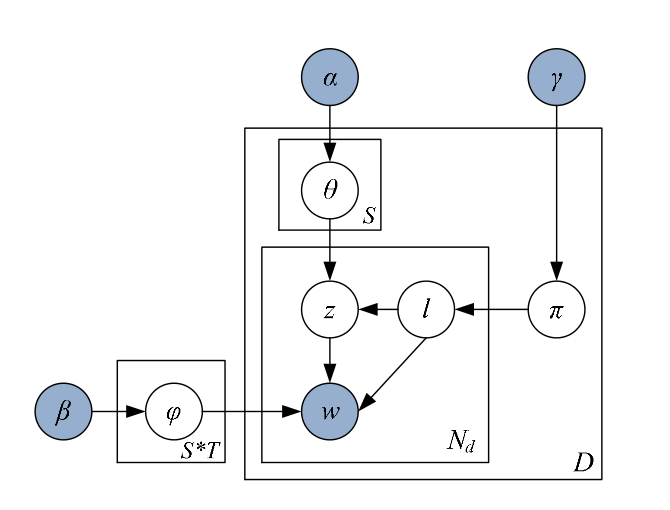
\includegraphics[width=\textwidth]{jst/jst.png} 
\begin{center}
 Figure 4.1 Joint Sentiment Topic Model
\end{center}

Assume that we have a collection of \(D\) documents denoted by \(C = {d_1,d_2,\cdots,d_D} \); each document in the corpus is a sequence
of \(N_d\) words denoted by \(d = (w_1,w_2,\cdots,w_{N_d}) \) and each word in the document is an item from a vocabulary index with V distinct
terms denoted by \({1,2,\cdots,V}\). Let \(S\) and \(T\) be the number of distinct sentiment and topic labels respectively. The procedure of
generating a document is described as follows.

\begin{alltt}
For each document \(d\), choose a distribution \(\pi_d \sim Dir(\gamma)\).
For each sentiment label \(l\) under document \(d\), choose a distribution
\(\theta_{d,k} \sim Dir(\alpha)\).
For each word \(w_i\) in document \(d\)
  - choose a sentiment label \(l_i \sim \pi_d\),
  - choose a topic \(z_i \sim \theta_{d,l_i}\),
  - choose a word \(w_i\) from the distribution over words defined by the 
    topic \(z_i\) and sentiment label \(l_i\), \(\psi_{z_i}^{l_i}\)
\end{alltt}

The hyper-parameter \(\alpha\) in \textit{JST} is the prior observation count for the number of times topic \(j\) is associated with 
sentiment label \(l\) sampled from a document. 

The hyper-parameter \(\beta\) is the prior observation count for the number of times words sampled from topic \(j\)
are associated with sentiment label \(l\).

Similarly, the hyper-parameter \(\gamma\) is the prior observation count for the number of times sentiment label \(l\) is associated
with a document.

The latent variables of interest in \textit{JST} are
\begin{enumerate}
 \item The joint sentiment/topic-document distribution, \(\theta\)
 \item The joint sentiment/topic-word distribution, \(\phi\)
 \item The joint sentiment-document distribution, \(\pi\)
\end{enumerate}

To obtain the distributions for \(\theta\), \(\phi\), and \(\pi\), we firstly estimate the posterior distribution over \(z\) i.e, the assignment
of word tokens to topics and sentiment labels.

We need to estimate the distribution, \(P(z_t=j,l_t=k|w,z_{\neg t},l_{\neg t},\alpha,\beta,\gamma)\) where \(z_{\neg t}\) and \(l_{\neg t}\)
are vector of assignments of topics and labels for all words in the collection except for the word position \(t\) in document \(d\). 

The joint distribution can be given as follows,
\begin{equation}
P(w,z,l) = P(w|z,l)P(z|l) = P(w|z,l)P(z|l,d)P(l|d)
\end{equation}

After calculations similar to \textit{LDA}, we get the following full conditional,

\begin{equation}
P(z_t=j,l_t=k|w,z_{\neg t},l_{\neg t},\alpha,\beta,\gamma) = 
\frac{\{N_{i,j,k}\}_{\neg t} + \beta}{\{N_{j,k}\}_{\neg t}+V\beta}.
\frac{\{N_{j,k,d}\}_{\neg t} + \alpha}{\{N_{k,d}\}_{\neg t}+T\alpha}.
\frac{\{N_{k,d}\}_{\neg t} + \gamma}{\{N_{d}\}_{\neg t}+S\gamma}
\end{equation}

where,

\(V\) is the size of the vocabulary \\
\(T\) is the number of topics \\
\(S\) is the total number of sentiment labels \\
\(D\) is the number of documents in the collection \\
\(N_{i,j,k}\) is the number of times word \(i\) appeared in topic \(j\) and with sentiment label \(k\) \\
\(N_{j,k}\) is the number of times words are assigned to topic \(j\) and sentiment label \(k\) \\
\(N_{j,k,d}\) is the number of times a word from document \(d\) has been associated with topic \(j\) and sentiment label \(k\) \\
\(N_{k,d}\) is the number of times sentiment label \(k\) has been assigned to some word tokens in document \(d\) \\
\(N_{d}\) is the total number of words in the collection \\

\par

\(\theta\), \(\phi\), and \(\pi\) can be estimated as follows

\begin{equation}
\phi_{i,j,k} = \frac{N_{i,j,k}+\beta}{N_{j,k}+V\beta}
\end{equation}

\begin{equation}
\theta_{j,k,d} = \frac{N_{j,k,d}+\alpha}{N_{k,d}+T\alpha}
\end{equation}

\begin{equation}
\pi_{k,d} = \frac{N_{k,d}+\gamma}{N_{d}+S\gamma}
\end{equation}

The Gibbs sampling procedure in this case is similar to that of \textit{LDA}. 

\par
\textit{JST} can be used for document level sentiment classification and topic detection simultaneously. \textit{Joint sentiment topic modeling}
is completely unsupervised as compared to existing approaches for sentiment classification. The performance of \textit{JST} on movie review
classification is competitive compared to other supervised approaches. \textit{JST} has been used in our experiments to compare it against our
approaches for sentiment analysis as explained in \cref{experiments}.

\section*{Summary}
In this chapter we explained how basic LDA can be used to perform the sentiment classification task. We also studied two models which combine sentiment
and topics. Both the systems have shown high competence in classification tasks. In the next chapter, we discuss the the topical n-gram model in detail.
We also explain how it can be used for sentiment classification.

\clearpage
% % Chapter Template

\chapter{Topical n-grams model} % Main chapter title

\label{topicalngram} % Change X to a consecutive number; for referencing this chapter elsewhere, use \ref{ChapterX}

\lhead{Chapter 5. \emph{Topical n-grams model}} % Change X to a consecutive number; this is for the header on each page - perhaps a shortened title

%----------------------------------------------------------------------------------------
%	Introduction
%----------------------------------------------------------------------------------------

Joint sentiment and topic models have been used to tackle this classification problem. Despite having a hierarchical structure, these generative models have
a bag of words assumption. Due to this fact, they tend to misclassify texts having sentiment in the form of phrases. \textit{LDA} and it's extensions don't 
work properly with phrases. To tackle this situation, we propose an unsupervised approach to sentiment analysis using the topical n-grams model which has been
shown to be effective with phrases. We train the topical n-grams model using two topics i.e., positive, and negative, list of positive and negative
words, and rules to detect positive and negative phrases. New documents are then classified using this trained model. The system gives better results than the 
existing Joint Sentiment Topic model. We also propose an approach to generate a list of positive and negative words using LDA based on our observations reported in~\cref{experiments}.

\section{Introduction}





In the next section, we will discuss the topical n-gram model in detail.

\section{Topical n-grams model}

n-gram phrases (or collocations) are fundamentally important in many areas of natural language processing (e.g., parsing, machine translation and information retrieval). 
Phrase as the whole carries more information than the sum of its individual components, thus it is much more crucial in determining the topics of document collections 
than individual words \citep*{wang2005note}. However, most of the topic models assume that words are generated independently to each other, i.e., under the bag of words
assumption. The possible over complicacy caused by introducing phrases makes these topic models completely ignore them. It is true that these models with the bag of words
assumption have enjoyed a big success, and attracted a lot of interests from researchers with different backgrounds. A topic model considering phrases would be more 
useful in certain applications. Topical n-grams model is one such generative model. It's generative process is explained as follows,

\begin{enumerate}
 \item Draw multinomial \(\phi_z\) from a Dirichlet prior \(\beta\);
 \item Draw binomial \(\psi_z\) from a Beta prior \(\gamma\);
 \item Draw multinomial \(\sigma_{zw}\) from a Dirichlet prior \(\delta\);
 \item For each document d, draw a multinomial \(θ^{(d)}\) from a Dirichlet prior \(\alpha\); then for each word \({w_i}^{(d)}\) in document \(d\),
    \begin{enumerate}
     \item Draw \({x_i}^{(d)}\) from binomial \(\psi_{{w_{i-1}}^{(d)}}\);
     \item Draw \({z_i}^{(d)}\) from multinomial \(\theta_{(d)}\);
     \item Draw \({w_i}^{(d)}\) from multinomial \(\sigma_{{w_{i-1}}^{(d)}}\) if \({x_i}^{(d)} = 1\); else draw \({w_i}^{d}\) from multinomial \(\phi_{{z_i}^{(d)}}\).
    \end{enumerate}
\end{enumerate}

The main point to infer from this generative process is that the topic assignments for the two terms in a bigram are not required to be identical. In the description of
topic n-grams given in \citep*{wang2005note}, they have used the topic of the last term as the topic of the phrase. But in our experiments, we have used certain rules
as prior information to assign topics to a phrase initially.


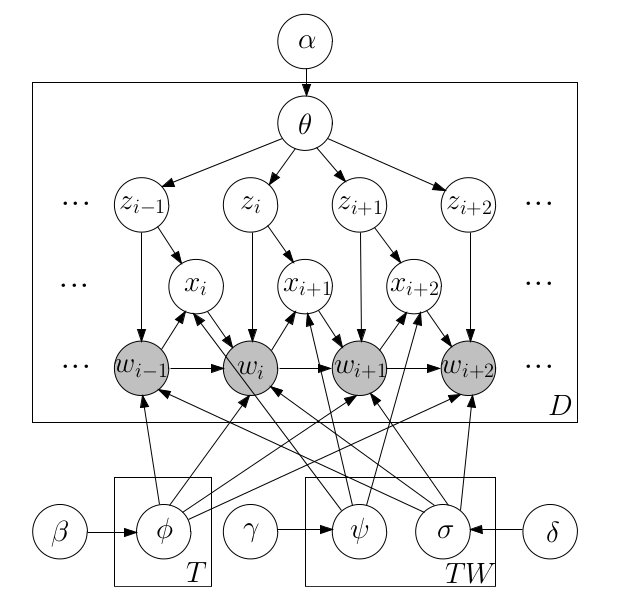
\includegraphics[width=\textwidth]{topicalngram.png} 
\begin{center}
 Figure 5.1 Topical n-grams model
\end{center}

\subsection{Inferencing}

Gibbs sampling is used to conduct approximate inference in this paper. During Gibbs sampling, we draw the topic assignment \(z_i\) and the bigram status \(x_i\) 
iteratively for each word \(w_i\) according to the following conditional probability distribution:

\begin{equation}
p(z_i,x_i | z_{-i},w_{-i},w,\alpha,\beta,\gamma,\delta) \propto
\frac{\gamma_{x_i} + p_{z_{i-1}w_{i-1}x_i}}{\sum_{k=0}^1 {(\gamma_k+p_{z_{i-1}}w_{i-1}k)}} {(\alpha_{z_i} + q_{d_{z_i}})} \times \left\{ 
  \begin{array}{l l}
    \frac{\beta_{w_i} + n_{z_i w_i}}{\sum_{v=1}^V {(\beta_v+n_{z_i v})}} & \quad \text{if $x_i$ is even}\\
    \frac{\delta_{w_i} + m_{z_i w_{i-1} w_i}}{\sum_{v=1}^V {(\delta_v + m_{z_i w_{i-1} v})} } & \quad \text{if $n$ is odd}
  \end{array} \right.
\end{equation}

where, 

\(z_{-i}\) denotes the topic assignments for all word tokens except word \(w_i\), \\ 
\(x_{-i}\) represents the bigram status for all tokens except word \(w_i\), \\ 
\(n_{zw}\) represents how many times word \(w\) is assigned into topic \(z\) as a unigram, \\
\(m_{zwv}\) represents how many tmes word \(v\) is assigned as the second term of a bigram given the previous word \(w\), \\
\(p_{zwk}\) denotes how many times the status variable \(x\) equals \(k\) given the previous word \(w\) and previous word's topic \(z\), and \\
\(q_{dz}\) represents how many times a word is assigned to topic \(z\) in document d.

In next section, we will explain the use of topical n-grams model for sentiment analysis

\section{Topical n-grams model for Sentiment Analysis}

To make use of topical n-grams model for sentiment classification, we use an approach similar to using LDA for sentiment classification.

\begin{itemize}
 \itemsep0em
 \item Set number of topics equal to 2.
 \item Remove stop-words.
 \item Remove objective words as they won't affect sentiment. The objective words in this case do not include the negation words like \textit{doesn't, 
 won't, no}, etc. This is to ensure that we can catch negation of polarity when they are used with subjective words.
 \item Apply Gibbs Sampling with prior. The prior used in this case is more sophisticated and can handle both words and phrases. In case of words, if
 is not present in a bigram then simply use a list of positive and negative words to assign positive or negative topic. If the word is present in a 
 bigram then assign it the topic of the bigram. There are some rules to detect and assign topics to bigrams which are explained next.
 \item Use the trained model to classify a new document as positive or negative.
\end{itemize}

\subsubsection*{Rules for Topic assignment of phrases}

At present, our rules are restricted to bigrams. We plan to extend them as explained in Section~\cref{conclusions}.
In the following rules, we mean topic when we say polarity. The use of polarity makes it easy to understand
the rules as they are concerned with subjectivity.

\begin{enumerate}
 \itemsep0em
 \item If the first word in the bigram is a negation word and the second word is subjective then the polarity
 of the bigram is opposite to the polarity of the second word. \\
 \textbf{Examples:} \textit{won't like, won't regret, etc.}. Here, \textit{won't like} is assigned negative
 polarity and \textit{won't regret} is assigned positive polarity.
 \item If both the words in the bigram are subjective then are two cases. If both words are of the same polarity
 then resultant polarity is the same. But if their polarities are different, then the polarity of the first word
 is assigned to the bigram. \\
 \textbf{Examples:} \textit{beautifully amazing} is positive as both words as positive. \textit{lack respect} is
 assigned negative as per the rules.
\end{enumerate}

One salient feature of this approach is that it is an unsupervised method and can work on any domain. 

\section*{SUMMARY}

In this chapter, we dicussed the motivation behind the topical n-grams model. Later on, we discussed the inference equation used by it. At the end,
we proposed an approach to use this model for sentiment analysis. The experiments and results obtained are discussed in ~\cref{experiments}.

In the next chapter, we will show the use of deep semantics for sentiement analysis.
% Chapter Template

\chapter{Deep Semantics for Sentiment Analysis} % Main chapter title

\label{unl} % Change X to a consecutive number; for referencing this chapter elsewhere, use \ref{ChapterX}

\lhead{Chapter 6. \emph{Deep Semantics for Sentiment Analysis}} % Change X to a consecutive number; this is for the header on each page - perhaps a shortened title

%----------------------------------------------------------------------------------------
%	SECTION 1
%----------------------------------------------------------------------------------------

Existing methods for sentiment analysis  use supervised approaches which take into account all the subjective words and or phrases. Due to this, the fact that not 
all of these words and phrases actually contribute to the overall sentiment of the \textit{text} is ignored. We propose an unsupervised rule-based approach using 
deep semantic processing to identify only relevant subjective terms. We generate a UNL (Universal Networking Language) graph for the input \textit{text}. Rules are
applied on the graph to extract relevant terms. The sentiment expressed in these terms is used to figure out the overall sentiment of the \textit{text}. Results on
binary sentiment classification have shown promising results.

\section{Introduction}

Many works in sentiment analysis try to make use of shallow processing techniques. The common thing in all these works is that they merely try to identify sentiment-bearing
expressions as shown by \citep*{ruppenhofer2012semantic}. No effort has been made to identify which expression actually contributes to the overall sentiment of the text. 
In \citep*{mukherjee2012sentiment} these expressions are given weight-age according to their position w.r.t. the discourse elements in the \textit{text}. But it still takes into 
account each expression.
 
Semantic analysis is essential to understand the exact meaning conveyed in the \textit{text}. Some words tend to mislead the meaning of a given piece of \textit{text} as
shown in the previous example. WSD (Word Sense Disambiguation) is a technique which can been used to get the right sense of the word. \citep*{balamurali2011harnessing} have 
made use of WordNet synsets for a supervised sentiment classification task. \citep*{martin2010word} and \citep*{rentoumi2009sentiment} have also shown a performance improvement 
by using WSD as compared to word-based features for a supervised sentiment classification task. In \citep*{saif2012semantic}, semantic concepts have been used as additional 
features in addition to word-based features to show a performance improvement. Syntagmatic or structural properties of text are used in many NLP applications like machine 
translation, speech recognition, named entity recognition, etc. A clustering based approach which makes use of syntactic features of text has been shown to improve performance 
in \citep*{arhaves}. Another approach can be found in \citep*{mukherjee2012sentiment} which makes use of lightweight discourse for sentiment analysis. In general, approaches 
using semantic analysis are expensive than syntax-based approaches due to the shallow processing involved in the latter. As pointed out earlier, all these works incorporate all 
the sentiment-bearing expressions to evaluate the overall sentiment of the \textit{text}. The fact that not all expressions contribute to the overall sentiment is completely 
ignored due to this. Our approach tries to resolve this issue. To do this, we create a UNL graph for each piece of \textit{text} and include only the relevant expressions to 
predict the sentiment. Relevant expressions are those which satisfy the rules/conditions. After getting these expressions, we use a simple dictionary lookup along with attributes
of words in a UNL graph to calculate the sentiment.

In the next section, we will go through some of the related work in this direction.

\section{Related Work}

There has been a lot of work on using semantics in sentiment analysis. \citep*{saif2012semantic} have made use of semantic concepts as additional features in a word-based 
supervised sentiment classifier. Each entity is treated as a semantic concept e.g. \textit{iPhone, Apple, Microsoft, MacBook, iPad, etc.}. Using these concepts as features, 
they try to measure their correlation with positive and negative sentiments. In \citep*{verma2009incorporating}, effort has been made to construct document feature vectors 
that are sentiment-sensitive and use world knowledge. This has been achieved by incorporating sentiment-bearing words as features in document vectors. The use of WordNet synsets 
is found in \citep*{balamurali2011harnessing}, \citep*{rentoumi2009sentiment} and \citep*{martin2010word}. The one thing common with these approaches is that they make use of 
shallow semantics. An argument has been made in \citep*{choi2008learning} for determining the polarity of a sentiment-bearing expression that words or constituents within the
expression can interact with each other to yield a particular overall polarity. Structural inference motivated by compositional semantics has been used in this work. This work 
shows use of deep semantic information for the task of sentiment classification. A novel use of semantic frames is found in \citep*{ruppenhofer2012semantic}. As a step towards 
making use of deep semantics, they propose SentiFrameNet which is an extension to FrameNet. A semantic frame can be thought of as a conceptual structure describing an event,
relation, or object and the participants in it. It has been shown that potential and relevant sentiment bearing expressions can be easily pulled out from the sentence using 
the SentiFrameNet. All these works try to bridge the gap between rule-based and machine-learning based approaches but except the work in \citep*{ruppenhofer2012semantic},
all the other approaches consider all the sentiment-bearing expressions in the text.

\section{Use of Deep Semantics}\label{deep}
Before devising any solution to a problem, it is advisable to have a concise definition of the problem. Let us look at the formal definition of the sentiment analysis 
problem as given in \citep*{liu2010sentiment}. Before we do that, let us consider the following review for a movie, \textit{"1) I went to watch the new James Bond flick, 
Skyfall at IMAX which is the best theater in Mumbai with my brother a month ago. 2) I really liked the seating arrangement over there. 3) The screenplay was superb 
and kept me guessing till the end. 4) My brother doesn’t like the hospitality in the theater even now. 5) The movie is really good and the best bond flick ever."}
This is a snippet of the review for a movie named Skyfall . There are many entities and opinions expressed in it. 1) is an objective statement. 2) is subjective but 
is intended for the theater and not the movie. 3) is a positive statement about the screenplay which is an important aspect of the movie. 4) is a subjective
statement but is made by the author’s brother and also it is about the hospitality in the theater and not the movie or any of its aspects. 5) reflects a positive
view of the movie for the author. We can see from this example that not only the opinion but the opinion holder and the entity about which the opinion has been expressed 
are also very important for sentiment analysis. Also, as can be seen from 1),4) and 5) there is also a notion of time associated with every sentiment expressed.
Now, let us define the sentiment analysis problem formally as given in \citep*{liu2010sentiment}.
  
\textit{A direct opinion about the object is a quintuple \(<o_j,f_{jk},oo_{ijkl},h_i,t_l>\), where \(o_j\) is the the object, \(f_{jk}\) is the feature of the object
\(o_j\), \(oo_{ijkl}\) is the orientation or polarity of the opinion on feature \(f_{jk}\) of object \(o_j\), \(h_i\) is the opinion holder and \(t_i\) is the time 
when the opinion is expressed by \(h_i\).}
  
As can be seen from the formal definition of sentiment analysis and the motivating example, not all sentiment-bearing expressions contribute to the overall sentiment
of the \textit{text}. To solve this problem, we can make use of semantic roles in the \textit{text}. Semantic role is the underlying relationship that the underlying
participant has with the main verb. To identify the semantic roles, we make use of UNL in our approach.
  
\subsection*{UNL (Universal Networking Language)}

UNL is declarative formal language specifically designed to represent semantic data extracted from natural language texts. In UNL, the information is represented by 
a semantic network, also called UNL graph. UNL graph is made up of three discrete semantic entities, Universal Words, Universal Relations, and Universal Attributes. 
Universal Words are nodes in the semantic network, Universal Relations are arcs linking UWs, and Universal attributes are properties of UWs. To understand UNL better, 
let us consider an example. UNL graph for \textit{"I like that bad boy"} is as shown in the figure.
  
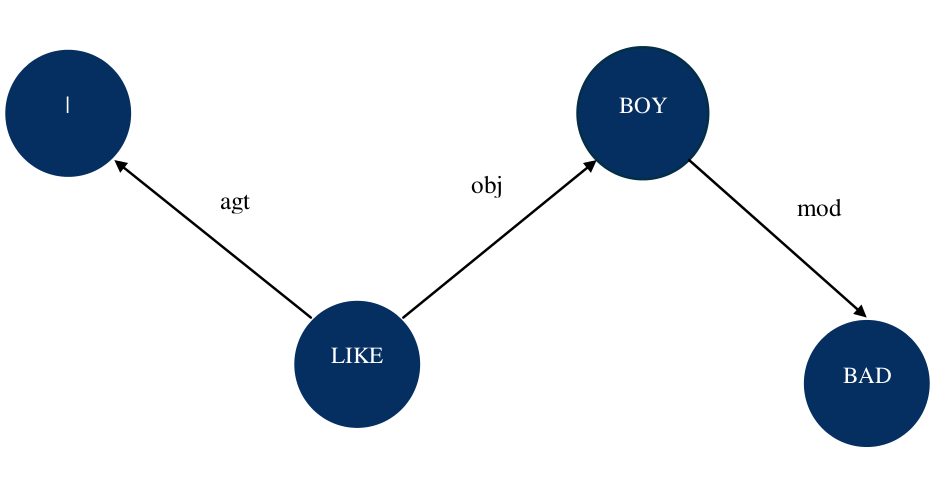
\includegraphics[width=\textwidth]{unlexample.png} 
\begin{center}
 Figure 6.1 UNL Example
\end{center}
  
Here, \textit{"I"}, \textit{"like"}, \textit{"bad"}, and \textit{"boy"} are the UWs. \textit{"agt"} (agent), \textit{"obj"} (patient), and \textit{"mod"} (modifier) are the
Universal Relations. Universal attributes are the properties associated with UWs which will be explained as and when necessary with the rules of our algorithm.
  
\subsubsection*{UNL relations}

Syntax of a UNL relation is as shown below,
    
\[\label{eqn:unlsyntax}
   <rel>:<scope><source>;<target>
\]
  
Where, \(<rel>\) is the name of the relation, \(<scope>\) is the scope of the relation, \(<source>\) is the UW that assigns the relation, and \(<target>\) is the UW that receives the relation \\
  
We have considered the following Universal relations in our approach,\\ 
1) \underline{\textit{agt} relation} \(:\) \textit{agt} stands for agent. An agent is a participant in action that provokes a change of state or location. The \textit{agt} 
relation for the sentence \textit{"John killed Mary"} is \textit{agt( killed , John )}. This means that the action of \textit{killing} was performed by \textit{John}.\\
2) \underline{\textit{obj} relation} \(:\) \textit{obj} stands for patient. A patient is a participant in action that undergoes a change of state or location. The \textit{obj} 
relation for the sentence \textit{"John killed Mary"} is \textit{obj( killed , Mary )}. This means that the patient/object of \textit{killing} is \textit{Mary}.\\
3) \underline{\textit{aoj} relation} \(:\) \textit{aoj} stands for object of an attribute. In the sentence \textit{"John is happy"}, the \textit{aoj} relation is 
\textit{aoj( happy , John )}.\\
4) \underline{\textit{mod} relation} \(:\) \textit{mod} stands for modifier of an object. In the sentence \textit{"a beautiful book"}, the \textit{mod} relation is 
\textit{mod( book , beautiful )}.\\
5) \underline{\textit{man} relation} \(:\) \textit{man} relation stands for manner. It is used to indicate how the action, experience or process of an event is carried out. 
In the sentence \textit{"The scenery is beautifully shot"}, the \textit{man} relation is \textit{man( beautifully , shot )}.\\
6) \underline{\textit{and} relation} \(:\) \textit{and} relation is used to state a conjunction between two entities. In the sentence \textit{"Happy and cheerful"}, 
the \textit{and} relation is \textit{and(Happy,cheerful)}.
    
\subsection*{Architecture}
  
As shown in the \textit{UNL} example, the modifier \textit{"bad"} is associated with the object of the main verb. It shouldn't affect the sentiment of the main agent. 
Therefore, we can ignore the modifier relation of the main object in such cases. After doing that, the sentiment of this sentence can be inferred to be positive.
The approach followed in the project is to first generate a UNL graph for the given input sentence. Then a set of rules is applied and used to infer the sentiment of the
sentence. The process is shown in Figure 6.2. The UNL generator shown in the Figure 6.2 has been developed at CFILT.\footnote{\url{http://www.cfilt.iitb.ac.in/}} Before, the given piece of text is passed on to the UNL 
generator, it goes through a number of pre-processing stages. Removal of redundant punctuations, special characters, emoticons, etc. are part of this process. This is
extremely important because the UNL generator is not able to handle special characters at the moment. We can see that, the performance of the overall system is limited
by this. A more robust version of the UNL generator will certainly allow the system to infer the sentiment more accurately.
  
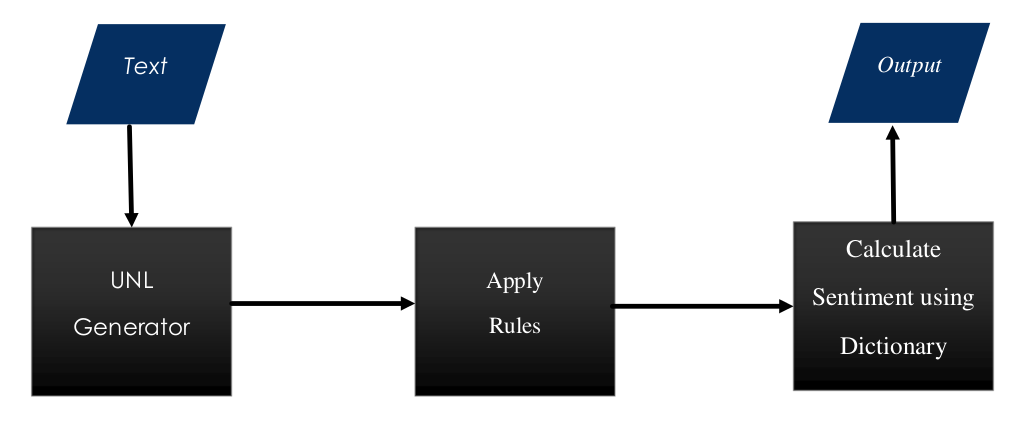
\includegraphics[width=\textwidth]{unlusage.png} 
\begin{center}
 Figure 6.2 Architecture
\end{center}
  
\subsection*{Rules}

There is a separate rule for each relation. For each UW (Universal word) considered, if it has a \textit{@not} attribute then its polarity is reversed. Rules used by the system
are as follows,\\
1) If a given UW is source of the \textit{agt} relation, then its polarity is added to the overall polarity of the text.
\underline{e.g.,} \textit{"I like her"}. Here, the agt relation will be \textit{agt ( like , I )}. The polarity of like being positive, the overall polarity of the text is positive.
\underline{e.g,} \textit{"I don't like her"}. Here the agt relation will be \textit{agt ( like@not , I )}. The polarity of like is positive but it has an attribute \textit{@not}
so its polarity is negative. The overall polarity of the text is negative in this case. \\
2) If a given UW is source or target of the \textit{obj} relation and has the attribute \textit{@entry} then its polarity is added to the overall polarity of the text. This rule 
merely takes into account the main verb of the sentence into account, and the it's is polarity considered.
\underline{e.g.,} \textit{"I like her"}, here the obj relation will be \textit{obj ( like@entry , her )}. The polarity of like being positive, the overall polarity of the text is positive \\
3) If a given UW is the source of the \textit{aoj} relation and has the attribute \textit{@entry} then its polarity is added to the overall polarity of the text.
\underline{e.g.,} \textit{"Going downtown tonight it will be amazing on the waterfront with the snow"}. Here, the \textit{aoj} relation is \textit{aoj ( amazing@entry , it )}. 
\textit{amazing} has a positive polarity and therefore overall polarity is positive in this case.\\
4) If a given UW is the target of the \textit{mod} relation and the source UW has the attribute \textit{@entry} or has the attribute \textit{@indef} then polarity of the 
target UW is added to the overall polarity of the text.
\underline{e.g.,} \textit{"I like that bad boy"}. Here, the aoj relation is \textit{mod ( boy , bad )}. \textit{bad} has a negative polarity but the source UW, boy does not have an 
\textit{@entry} attribute. So, in this case negative polarity of bad is not considered as should be the case.
\underline{e.g.,} \textit{"She has a gorgeous face"}. Here, the mod relation is \textit{mod ( face@indef , gorgeous )}. \textit{gorgeous} has a positive polarity and face has an 
attribute \textit{@indef}. So, polarity of gorgeous should be considered. \\
5) If a given UW is the target of the \textit{man} relation and the source UW has the attribute \textit{@entry} then polarity of the target UW is added to the overall polarity of 
the text. Or if the target UW has the attribute \textit{@entry} then also we can consider polarity of the target UW. 
\underline{e.g.,} \textit{"He always runs fast"}. Here, the \textit{aoj} relation is \textit{mod ( run@entry , fast )}. \textit{fast} has a positive polarity and the source UW, run 
has the \textit{@entry} attribute. So, in this case positive polarity of fast is added to the overall polarity of the sentence.
Polarities of both the source and target UW of the \textit{and} relation are considered. \\
6) In \textit{"Happy and Cheerful"}, the \textit{and} relation is \textit{and(Happy, Cheerful)}. \textit{Happy} and \textit{Cheerful}, both have a positive
polarity, which gives this sentence an overall positive polarity.
 
The polarity value of each individual word is looked up in a dictionary of positive of negative words used is \citep*{liu2010sentiment} After all the rules are applied, summation of all the calculated polarity values is done. 
If this sum is greater than 0 then it is considered as positive, and negative otherwise. This system is negative biased due to the fact that people often tend to express negative sentiment 
indirectly or by comparison with something good.

\section*{SUMMARY}

In the beginning, we expressed the motivation behind this approach. After that, related work was discussed. Then we explained the approach to use deep semantics in detail.
The experiments performed using this approach will be explained in the next chapter.
% \chapter{Experiments} % Main chapter title

\label{experiments} % For referencing the chapter elsewhere, use \ref{Chapter5} 

\lhead{Chapter 5. \emph{Experiments}} % This is for the header on each page - perhaps a shortened title

%----------------------------------------------------------------------------------------


In this chapter, we will show how \textit{LDA} was evaluated to test the accuracy of unsupervised approaches in general. Then, the use of topic
models to perform the sentiment classification task is explained. At the end, the system using deep semantics is explained.

\section{Evaluation of LDA}

Evaluation of topic models has been discussed at length in \citep*{wallach2009evaluation}. A natural evaluation metric discussed in 
\citep*{wallach2009evaluation} is finding out the probability of a held-out document given a trained model. Topic modeling is a useful
tool for analyzing unstructured text collections. Evaluation of topic models is difficult due to their unsupervised nature. For some 
applications, there might be extrinsic tasks such as information retrieval for which performance can be evaluated. There is a need for 
a universal method that measures generalization capability of a topic model in a way that is accurate, computationally efficient and
independent of a specific application. \textit{LDA} can be evaluated by 1) Information retrieval accuracy or 2) by estimating the probability
of unseen held-out documents given some training documents. We propose a new evaluation method as follows.

\subsection*{Evaluation method}

\begin{enumerate}
 \item Download documents.
 \item Tag every document with a topic to get a tagged corpus
 \item Held-out some documents for testing before training the model
 \item Train the topic model using the untagged corpus (obtained after removing the tags)
 \item Now, use the trained model to infer topic distribution for the testing documents
 \item Check whether the topic having highest proportion matches the tag of the document
\end{enumerate}

5-fold cross validation was used in this case. 1273 documents were downloaded from DMOZ \citep*{dmoz}. Computers, films, real estate, cooking and
sports were the 5 topics chosen. The implementation in Mallet was used to conduct the experiment.

\begin{center}
\begin{tabular}{ |c|c| }
  \hline
  Topic & No. of files \\ \hline
  Computers & 164 \\ \hline
  Sports & 213 \\ \hline
  Cooking & 251 \\ \hline
  Real Estate & 261 \\ \hline
  Films & 384 \\ \hline
\end{tabular}
\end{center}
\begin{center}
 Table 7.1 Number of files per topic
\end{center}

\begin{center}
\begin{tabular}{ |c|c| }
  \hline
  Average accuracy & 20.867 \\ \hline
\end{tabular}
\end{center}
\begin{center}
 Table 7.2 Average Accuracy 
\end{center}

\subsection*{Discussion}

\par
The average accuracy after 5-fold cross-validation on this corpus was 20.867, which is very low. The reason for this is the short-length
of the documents used. \textit{LDA} works on the principle of co-occurrence. If we look at \eref{eqn:fullconditionalfinal}, there is a
factor for words and another for documents. Probabilities are higher for assignments that "don't break document boundaries", that is, words 
appearing in the same document have a slightly higher odds of ending up in the same topic. The same holds for document assignments, they to 
a degree follow "word boundaries". These effects mix up and spread over clusters of documents and words, eventually. Due to the short length 
of the documents, words from the same topic may not always co-occur. Also, there is chance of them co-occurring with words from other topics 
also which results in bad clustering. Some words belong to more than one topic due to this. Due to this, the clustering of documents as whole 
in this case is not good. 

\par
Also, the evaluation method used is very strict. If it is a bit lenient, the accuracy can be increased. A new method
called weighted evaluation can be used in this case.

\subsection*{Weighted Evaluation}

Weighted evaluation is based on the fact that we get a topic distribution for each testing document. This topic distribution is arranged
in descending order of topic proportions. The idea is to assign weights according to the rank given to the original tag of the document. 

\subsection*{Weighted Evaluation Algorithm}

\begin{alltt}
matches=0, counts=0
For each document
  Find topic distribution
  Switch(tag):
    case(topic1): matches += 1
    case(topic2): matches += 0.8
    case(topic3): matches += 0.6
    case(topic4): matches += 0.4
    case(topic5): matches += 0.2
    counts++
Accuracy = matches/counts
\end{alltt}

\subsection*{Results}

\begin{center}
\begin{tabular}{ |c|c|c|c| }
  \hline
  Fold & Matches & Counts & Accuracy (in percentage) \\ \hline
  Fold 1 & 156 & 255 & 61.4 \\ \hline
  Fold 2 & 156 & 255 & 61.4 \\ \hline
  Fold 3 & 170 & 255 & 66.9 \\ \hline
  Fold 4 & 152 & 255 & 59.6 \\ \hline
  Fold 5 & 161 & 253 & 63.9 \\ \hline
\end{tabular}
\end{center}
\begin{center}
 Table 7.3 Accuracy for each testing fold 
\end{center}

\begin{center}
\begin{tabular}{ |c|c| }
  \hline
  Average accuracy & 62.6 \\ \hline
\end{tabular}
\end{center}
\begin{center}
 Table 7.4 Weighted Evaluation Average Accuracy 
\end{center}

\subsection*{Discussion}

\par
As we can see the accuracy has increased after we used weighted evaluation. This kind of evaluation needs to be used in many systems including
transliteration where the most probable word needs to be predicted. The rank of the actual word may be further down. This doesn't mean that the
system is giving wrong output. Therefore, a more lenient approach would be better in this case. 

\par
The accuracy has increased but still is unsatisfactory. 62 \% accuracy in this case implies that given a document, there is 62 \%
chance that the main topic of the document will be ranked in top 5. As we have used only 5 topics, this result is not that significant. Using
more number of topics will lead to better insights. 

\par 
If we consider the clustering to be effective only till the third rank, we get accuracies as shown in the table.

\begin{center}
\begin{tabular}{ |c|c|c|c| }
  \hline
  Fold & Matches & Counts & Accuracy (in percentage) \\ \hline
  Fold 1 & 156 & 255 & 50.9 \\ \hline
  Fold 2 & 156 & 255 & 50.1 \\ \hline
  Fold 3 & 170 & 255 & 57.4 \\ \hline
  Fold 4 & 152 & 255 & 46.7 \\ \hline
  Fold 5 & 161 & 253 & 53.5 \\ \hline
\end{tabular}
\end{center}
\begin{center}
 Table 7.5 Accuracy for each testing fold (Till 3rd rank)
\end{center}

\begin{center}
\begin{tabular}{ |c|c| }
  \hline
  Average accuracy & 51.7 \\ \hline
\end{tabular}
\end{center}
\begin{center}
 Table 7.6 Average Accuracy (Till 3rd rank)
\end{center}

\par 

This means that given a document, there is 51.7 \% chance that the main topic of the document will be ranked in top 3. It is known
that \textit{LDA} performs better with more number of topics. So, increasing the number of topics while performing the evaluation can 
lead to more better results. 

A list of high probability words for each topic was prepared which is given in the following table. 

\begin{center}
\begin{tabular}{ |c|c|c|c|c| }
  \hline \hline
  Computer & Films & Cooking & Real Estate & Sports \\ \hline \hline
  site & film &	recipes & services & reviews \\ \hline
  software & information & recipe & real & news \\ \hline
  free & offers & including & company &	interviews\\ \hline
  systems & production & collection & estate & information \\ \hline
  programming & courses & tips & includes & features \\ \hline
  research & links & source & commercial & current \\ \hline
  resources & videos & production & based & tennis \\ \hline
  code & television & baking & development & running \\ \hline
  information &	cinema & breakfast & title & tournament \\ \hline
\end{tabular}
\end{center}
\begin{center}
 Table 7.7 High probability words in each topic 
\end{center}

As we can see, the high probability words in each topic are good but due to the short length, results were not that good. 

\section{Using Topic models for Sentiment Analysis}

Analysis was performed for the binary sentiment classification task. The language used in this case was English.
We conducted experiments on 4 models, BOW using SVM, LDA ~\citep*{blei2003latent}, JST ~\citep*{lin2009joint}, and 
Topical n-gram model ~\citep*{wang2007topical}. We used two settings for the topic models, with and without prior. 
The word lists used are those specified in ~\citep*{liu2010sentiment}. The implementations of SVM, LDA and Topical
n-gram in Mallet \footnote{http://mallet.cs.umass.edu/} have been used for evaluation. For JST, we have used the 
implementation provided by the authors \footnote{https://github.com/linron84/JST}. The default settings for the
hyper-parameters were used in all these implementations. Some changes in the implementations of LDA and Topical
n-gram were made to take into account the prior information.

\subsection*{Dataset}

To create the dataset we used the amazon reviews dataset provided by SNAP \footnote{http://snap.stanford.edu/}.
These reviews are not tagged with sentiment but they have ratings from 1 to 5. We used this information to create
a sentiment tagged corpus. The reviews with ratings less than 3 were tagged as negative and others were tagged
as positive. We conducted the experiments on 6,00,000 reviews containing equal number of positive and negative
reviews.

\subsection*{Results}\label{results}

The results presented here are for 10-fold cross validation. For the topic models, due to the randomness involved 
during sampling, the best result obtained for each fold has been used for calculating the average. The Bag of words 
system performs better than all the models when no prior information is provided. The performance of topic models 
significantly increases when prior information is provided. Our approach to use Topical n-gram outperforms all the 
systems when a prior is used.

\begin{center}
\begin{tabular}{|l|c|}
\hline \bf System & \bf Avg. accuracy (\%)\\ \hline
BOW-SVM & 82.45\\
LDA & 65.34\\
LDA with prior & 80.19\\
JST & 68.64\\
JST with prior & 84.43\\
Topical n-gram & 63.57\\
Topical n-gram with prior & \textbf{87.32}\\
\hline
\end{tabular}
\end{center}
\begin{center}
 Table 7.8 Evaluation of Topic models for Binary sentiment classification.
\end{center}

\subsection*{Discussion}\label{discussion}

The performance of our system is better due to the capacity to handle phrases. All the other systems, consider each word
separately. The performance improvement over JST is 3\% which is statistically significant. Though the system performs
better for this dataset, it still has some obvious limitations. The system highly depends on the rules used for
initial assignment of topics which is evident from the results. These rules don't apply to all the bigrams. Let us
consider, the bigram \textit{insanely good}. In this case, the first word is negative and second word is positive. The rules
will assign a negative polarity to this bigram. But in this phrase \textit{insanely} is used to increase the intensity of 
\textit{good}. The rules apply only for bigrams, we need to add more rules to handle n-grams. A phrase like \textit{I don't
think it's good} won't be handled by the system. During error analysis, we also found that some words like \textit{engrossing,
blockbuster, bravo, etc.}, are not present in the word lists. These words convey a positive sentiment but our system fails
to correctly classify reviews containing such words. Also, words like \textit{awsome} which is spelling mistake of \textit{awesome}
are often found in reviews. We thought that the accuracy might be increased if we could detect the correct subjective
nature of these words and also the bigrams using them. For this, we proposed  an approach for resource generation using LDA.

The word lists we generated using this approach were used to test the systems using priors. The results for the same
are shown in Table 2. We can see a marginal increase in the accuracy in this setting.

\begin{center}
\begin{tabular}{|l|c|}
\hline \bf System & \bf Avg. accuracy (\%)\\ \hline
LDA with prior & 80.21\\
JST with prior & 86.37\\
Topical n-gram with prior & \textbf{89.83}\\
\hline
\end{tabular}
\end{center}
\begin{center}
 Table 7.9 Evaluation using resources generated using \textit{LDA}
\end{center}

In the next section, we explain the experiments done using deep semantics.

\section{Deep Semantics for sentiment analysis}

Analysis was performed for monolingual binary sentiment classification task. The language used in this case was \textit{English}. The comparison was done between 5 systems 
viz. System using words as features, WordNet sense based system as given in \citep*{balamurali2011harnessing}, Clusters based system as described in ~\citep*{arhaves}, 
Discourse rules based system as given in \citep*{mukherjee2012sentiment}, and the UNL rule based system. Two polarity datasets were used to perform the experiments. 
    
\begin{enumerate}
  \item \underline{EN-TD:} English Tourism corpus as used in \citep*{ye2009sentiment}. It consists of 594 positive and 593 negative reviews.
  \item \underline{EN-PD:} English Product (music albums) review corpus \citep*{blitzer2007biographies}. It consists of 702 positive and 702 negative 
  reviews. 
\end{enumerate}
   
For the WordNet sense, and Clusters based systems, a manually sense tagged version of the (EN-PD) has been used. Also, a automatically sense tagged version of 
(EN-TD) was used on these systems. The tagging in the later case was using an automated WSD engine, trained on a tourism domain \citep*{balamurali2013lost}.
The results reported for supervised systems are based on 10-fold cross validation.
   
\subsection*{Results}\label{results}

\begin{center}
  \begin{tabular}[h]{|l|c|c|}
   \hline
   \textbf{System} & \textbf{EN-TD} & \textbf{EN-PD} \\ \hline \hline
   Bag of Words & 85.53 & 73.24 \\ \hline
   Synset-based & 88.47 & 71.58 \\ \hline
   Cluster-based & \textbf{95.20} & 79.36 \\ \hline
   Discourse-based & 71.52 & 64.81 \\ \hline
   UNL rule-based & 86.08 & \textbf{79.55} \\ \hline
   \hline
  \end{tabular}
\end{center}
\begin{center}
 Table 7.10 Classification accuracy (in \%) for monolingual binary sentiment classification
\end{center}

  
The results for monolingual binary sentiment classification task are shown in Table ~\ref{table:accuracy}. The results reported are the best results obtained in 
case of supervised systems. The cluster based system performs the best in both cases. The UNL rule-based system performs better only than the bag of words
and discourse rule based system. For EN-PD ( music album reviews ) dataset, the UNL based system outperforms every other system . These results are very promising 
for a rule-based system. The difference between accuracy for positive and negative reviews for the rule-based systems viz. Discourse rules based and UNL rules based 
is shown in Table ~\ref{table:accuracyposneg}. It can be seen that the Discourse rules based system performs slightly better than the UNL based system for positive 
reviews. On the other hand, the UNL rules based system outperforms it in case of negative reviews by a huge margin. 
  
\begin{center}
  \begin{tabular}[h]{l|c|c|c|c|}
   \cline{2-5}
    & \multicolumn{2}{|c|}{\textbf{EN-TD}} & \multicolumn{2}{|c|}{\textbf{EN-PD}} \\ \hline
    \textbf{System} & \textbf{Pos} & \textbf{Neg} & \textbf{Pos} & \textbf{Neg} \\ \hline \hline
    Discourse rules & 94.94 & 48.06 & \textbf{92.73} & 36.89 \\ \hline
    UNL rules & \textbf{95.72} & \textbf{76.44} & 90.75 & \textbf{68.35} \\ \hline
   \hline
  \end{tabular}
\end{center} 
\begin{center}
 Table 7.11 Classification accuracy (in \%) for positive and negative reviews
\end{center}

\subsection*{Discussion}

The UNL generator used in this case is the bottleneck in terms of performance. Also, it makes use of the standard NLP tools viz. parsing, co-reference resolution, etc. 
to assign the proper semantic roles in the given \textit{text}. It is well known fact that these techniques work properly only on structured data. The language used in 
the reviews present in both the datasets is unstructured in considerable number of cases. The UNL generator is still in its infancy and cannot handle \textit{text} 
involving special characters. Due to these reasons, a proper UNL graph is not generated in some cases. Also, it is not able to generator proper UNL graphs for even well 
structured sentences like \textit{"It is not very good"}. In this case, the UW,  \textit{good} should have an attribute \textit{@not} which implies that it is used in 
a negative sense. On the contrary, the UNL generator does not assign any such attribute to it, leading to incorrect classification. As a result of all these things, the 
classification accuracy is low.

Negative reviews have certain characteristics which make them difficult to classify. Sentences like \textit{"It is good but could be better"} are very common in negative 
reviews. Some reviews are just to raise caution. A negative review about \textit{Las Vegas} contained the sentence, \textit{"Do not go to Las Vegas alone if you are female"}. 
Some reviews contain mixed opinions. For example, \textit{"Beautiful Architecture. Expensive food"}. We stated the importance of time in sentiment analysis in \cref{unl}. 
Examples of such a sentence is \textit{"A place I used to love. Not anymore"}. To infer that the sentence, \textit{"The hotel room had a Queen-sized bed"} has a negative 
sentiment is not possible without proper domain knowledge. Sentiment is domain dependent as given in ~\citep*{liu2010sentiment}. The adjective \textit{cheesy} might be positive for a 
food item but is definitely negative in cases like \textit{"The place is full of cheesy shows"}. Reviewers often criticize a place/thing by praising other places/things. In 
the EN-TD dataset, negative reviews were full of sentences like \textit{"If you want dirt, go to L.A. . If you want peace, go to Switzerland."}. \textit{"I love New York 
especially the 'Lovely brown fog'"} and \textit{"I adore the 'phony fantasy-land' that Vegas is"} are examples of sarcasm. Sarcasm is a very difficult problem to tackle. 
Some related works can be found in ~\citep*{carvalho2009clues} and ~\citep*{gonzalez2011identifying}.

In some cases, the reviewers make use of their native language and expressions. This is a big problem for the task of monolingual sentiment classification. From this discussion, it is clear that two major points of concern are unstructured language and hidden sentiment

\section*{Summary}

In this chapter, we first evaluated \textit{LDA} for the binary sentiment classification task. After that, we evaluated the topic models in different settings against
each other and the bag of words model. The system using deep semantics was compared with some state of the art systems for the same task but a different dataset.

In the next chapter, we conclude and comment on some future work.

\clearpage 
% Chapter 6

\chapter{Conclusions and Future Work} % Main chapter title

\label{conclusions} % For referencing the chapter elsewhere, use \ref{Chapter6} 

\lhead{Chapter 6. \emph{Conclusions and Future Work}} % This is for the header on each page - perhaps a shortened title

%----------------------------------------------------------------------------------------

\section{Conclusion}

A wide variety of approaches have been used for detecting sentiment in \textit{text}. Supervised, Unsupervised and semi-supervised methods have been 
explored to solve this difficult problem. Due the unstructured nature of the \textit{text} used for sentiment analysis, standard \textit{NLP} tools 
cannot be used directly. This has lead many techniques to make use of bag-of-words like models which makes strong independence assumptions. The accuracy
of bag-of-words model is less than desirable. So, this model is augmented with information about coherency, discourse, and pragmatics if it is present 
in the \textit{text}. Graph based formulation has become really important to encode this information in the feature vector as it is very difficult to 
encode it in the standard \textit{ML} techniques discussed. Domain dependence of sentiment also plays a very crucial role in sentiment analysis. A complete
reversal of sentiment orientation is observed in some cases. Problems like sarcasm and thwarting still persist and no clear solution is present at the moment. 

\textit{Information Retrieval} is mostly concerned with factual data. Using subjectivity analysis, subjective \textit{text} can be filtered out. This can 
remove \textit{text} containing opinion of the author. But in some cases, retrieval of subjective text is very important. For example, you might want to 
fetchall reviews related to a product. This is called sentiment aware \textit{IR}. In information retrieval, corpus modeling has been used extensively over
the years to fetchdocuments related to a specific topics. The topics of interest are expressed by the words in the query. Topic modeling approach can be 
extended to model the sentiment of the \textit{text}. When these two models are combined, not only does it help in fetching \textit{text} pertaining to certain
topics but also of the desired sentiment. Though these models make strong independence assumptions, their combination helps to model topic dependence of 
sentiment by encoding co-occurrence between sentiment and topic words. \textit{Sentiment Analysis} and \textit{Information Retrieval} can be combined to 
achieve very good results in sentiment aware information retrieval.

Topical n-gram model can be used for the binary sentiment classification problem. The motivation behind this approach was to use not only words but also 
phrases to classify documents. The model was trained with documents containing only subjective and negation words and bigrams formed by the combination of 
these. It also made use of rules to assign topics to words and bigrams in the intialization stage of estimation. Results using a prior show statistically 
significant improvement over the JST model. The paper also shows the use of LDA for resource generation, prompted by observations made during error analysis. 
The system shows marginal improvement in accuracy after using the resources generated by this technique.

Using deep semantics for sentiment analysis of structured data increases classification accuracy sentiment analysis. A semantic role labeling method through 
generation of a UNL graph was used to do this. The main motivation behind this research was the fact that not all sentiment bearing expressions contribute to
the overall sentiment of the \textit{text}. The approach was evaluated on two datasets and compared with successful previous approaches which don't make use 
of deep semantics. The system underperformed all the supervised systems but showed promise by yielding better results than the other rule-based approach. Also, 
in some cases the performance was very close to the other supervised systems. The system works well on sentences where are inherently complex and difficult 
for sentiment analysis as it makes use of semantic role labeling. Any rule based system can never be exhaustive in terms of rules. We always need to add new 
rules to improve on it. In some case, adding new rules might cause side-effects. In this case, as the rules are intuitive, adding of new rules will be easy. 
Also, analysis of the results hints at some ways to tackle specific problems effectively.

\section{Future work}

\subsection{Short term}
The system using topical n-grams model is focused on bigrams at the moment. It can be extended to handle n-grams by adding rules to detect and assign topics. 
Instead of adding rules, we can make use of machine learning techniques to detect the subjective nature of a phrase. For the \textit{UNL} system, Adding more 
rules to the system will help to improve the system. Language gets updated almost daily, we plan to update our dictionary with these new words and expressions 
to increase the accuracy. Also, we plan to replace the UNL system with a dependency parsing system and apply rules similar to the ones described in this work.

\subsection{Medium term}
As both the systems have shown increase in accuracy, a combination of topic models and semantics should be done.

\subsection{Long term}

% Unstructured nature of the \textit{text} mostly involved in sentiment analysis is a very big obstacle. This makes it difficult
% to take into account discourse and pragmatics. There is shortage of work which consider these important elements of textual data.
% Graph based solutions to these problems have been discussed. Most of the future work in \textit{SA} will focus on how to integrate this
% information in the feature vector so that it results in better classification.
% 
% Strong independence assumptions as we saw might mislead the classifier. Instead of using the same type of corpus modeling used 
% in many \textit{IR} applications, effort should be made to embed discourse and pragmatics information into the model. This will improve
% the accuracy of sentiment aware \textit{IR} systems. 


%----------------------------------------------------------------------------------------
%	THESIS CONTENT - APPENDICES
%----------------------------------------------------------------------------------------

\addtocontents{toc}{\vspace{2em}} % Add a gap in the Contents, for aesthetics

\appendix % Cue to tell LaTeX that the following 'chapters' are Appendices

% Include the appendices of the thesis as separate files from the Appendices folder
% Uncomment the lines as you write the Appendices

%% Appendix A

\chapter{Appendix Title Here} % Main appendix title

\label{AppendixA} % For referencing this appendix elsewhere, use \ref{AppendixA}

\lhead{Appendix A. \emph{Appendix Title Here}} % This is for the header on each page - perhaps a shortened title

Write your Appendix content here.
%\input{./Appendices/AppendixB}
%\input{./Appendices/AppendixC}

\addtocontents{toc}{\vspace{2em}} % Add a gap in the Contents, for aesthetics

\backmatter

%----------------------------------------------------------------------------------------
%	References
%----------------------------------------------------------------------------------------

\label{References}

\lhead{\emph{References}} % Change the page header to say "Bibliography"

\bibliographystyle{unsrtnat} % Use the "unsrtnat" BibTeX style for formatting the Bibliography

\bibliography{Bibliography} % The references (bibliography) information are stored in the file named "References.bib"

\end{document}  